% TODO: include fluctuating loads here and make it transparent
% %\usepackage[left=2cm,right=2cm,top=2cm,bottom=2cm]{geometry}
%

\documentclass{beamer}

% language
%\usepackage[ngerman]{babel}   % include for German presentations

% font encryption
\usepackage[T1]{fontenc}
\usepackage[utf8]{inputenc}
%\usepackage[latin1]{inputenc}

% styles
\usepackage{multimedia}
\usepackage{tabularx}

% figures
\usepackage{natbib} 
\usepackage{subfig}
\usepackage{color} 
\usepackage{graphicx}
\usepackage{graphics}
\usepackage{epsfig}

% necessary packages for layout
\usepackage{beamerthemesplit}
\usepackage{watermark}
\usepackage{helvet} % fonttype

% math package
\usepackage{amsmath}
\usepackage{amsfonts}
\usepackage{mathtools}
\everymath{\displaystyle} % avoids smaller math fonts of fractions

%tikz
\usepackage{tikz,pgfplots}
\usetikzlibrary{calc,intersections,through,backgrounds,decorations.text,patterns}
\usetikzlibrary{decorations.pathreplacing,decorations.markings}


\usepackage{amsmath}
\usepackage{amsfonts}
\usepackage{amssymb}
\usepackage{tikz}
\usetikzlibrary{shapes}
\usetikzlibrary{arrows}
\usetikzlibrary{positioning}
\usetikzlibrary{decorations.markings}
\usepackage{bm}
\usepackage{makeidx}
\usepackage{graphicx}
\usepackage{caption}
\usepackage{subfig}
\usepackage{siunitx}
\usepackage{accents}
\newcommand*{\dt}[1]{%
	\accentset{\mbox{\large\bfseries .}}{#1}}
\usepackage{float}
%\usepackage[backend= bibtex,sorting=none,citestyle=numeric,bibstyle=numeric]{biblatex}
%\usepackage[left=2cm,right=2cm,top=2cm,bottom=2cm]{geometry}
\usepackage[absolute,overlay]{textpos}

%\usepackage{pstricks}
%\usepackage{pst-fill,pst-grad}
%\usepackage{pst-text}
%\usepackage{pst-uml}
\usepackage{pdfpages}
%\usepgfplotslibrary{external}
%\tikzexternalize
%\tikzsetexternalprefix{external_figs/}
\pgfplotsset{compat=newest}
%% the following commands are needed for some matlab2tikz features
\usetikzlibrary{plotmarks}
\usetikzlibrary{arrows.meta}
%\usepgfplotslibrary{patchplots}
\usepackage{grffile}

\usepackage{tabularx}

\usetikzlibrary{matrix,positioning,decorations.pathreplacing}
\DeclareMathOperator{\Mcol}{col}
\DeclareMathOperator{\Mrow}{row}
\DeclareMathOperator{\Mnull}{null}
%\usepackage[latin1]{inputenc}
\usetikzlibrary{shapes,arrows}
%%\usepackage[active,tightpage,pdftex]{preview}
%\usepackage{mathtools}
%\usepackage{pgfplots}
%\usepackage{siunitx}
%
%\usepackage{tikz}
\usetikzlibrary{shapes}
\usetikzlibrary{calc}
\usepackage{setspace}% http://ctan.org/pkg/setspace

\usepackage{animate}
\usepackage{media9}
\usepackage[]{algorithm2e}
\usepackage{amsmath,amsthm,amstext,amssymb}
%\usepackage[export]{adjustbox}
\usepackage{multimedia}
\usepackage{animate}
\usepackage{xmpmulti}

\usefonttheme{professionalfonts}
\setbeamerfont{title}{series=\bfseries}
\setbeamerfont{subtitle}{series=\mdseries}
\setbeamerfont{frametitle}{series=\mdseries}
\setbeamerfont{footline}{series=\mdseries}%, size=\scriptsize}
\linespread{1.2}

\definecolor{luhBlue}{RGB}{0,80,155}
\definecolor{luhBlue40}{RGB}{153,185,216}
\definecolor{luhBlue20}{RGB}{204,220,235}
\definecolor{luhGreen}{RGB}{200,211,23}
\definecolor{darkGray}{RGB}{153,153,153}
\definecolor{lightGray}{RGB}{204,204,204}

\setbeamercolor{title}{fg=luhBlue}
\setbeamercolor{subtitle}{fg=luhBlue40}
\setbeamercolor{titlelike}{fg=luhBlue,parent=structure}
\setbeamercolor{titlelike}{fg=luhBlue,bg=}
\setbeamercolor{normal text}{fg=black}
\setbeamercolor{alerted text}{fg=luhGreen}
\setbeamercolor{example text}{fg=luhBlue20}
\setbeamercolor{structure}{fg=black}

\setbeamercolor{itemize item}{fg=darkGray}
\setbeamercolor{itemize subitem}{fg=darkGray}
\setbeamercolor{itemize subsubitem}{fg=darkGray}

\setbeamercolor{item projected}{fg=white,bg=darkGray}
\setbeamercolor{enumerate subitem}{fg=darkGray}
\setbeamercolor{enumerate subsubitem}{fg=darkGray}

\setbeamertemplate{itemize items}[ball]
\setbeamertemplate{items}[ball]

% Blocks
%\setbeamercolor{block body}{fg=black,bg=white}
%\setbeamercolor{block body alerted}{fg=black,bg=white}
%\setbeamercolor{block body example}{fg=black,bg=white}
\setbeamercolor{block title}{fg=white,bg=luhBlue}
\setbeamercolor{block title alerted}{use={normal text,alerted text},fg=black,bg=luhGreen}
\setbeamercolor{block title example}{use={normal text,example text},fg=black,bg=luhBlue40}

% Layout
\useinnertheme{rectangles} % rectangles circles
\beamertemplatenavigationsymbolsempty
%\setbeamercovered{transparent} % hidden content is transparent
%\setbeamercovered{invisible} % hidden content is invisible
\setbeamercolor{section number projected}{bg=darkGray,fg=white}
\setbeamercolor{subsection number projected}{bg=darkGray,fg=white}

% headline design
\setbeamertemplate{headline}{
\begin{picture}(0,-10)(-230,30)
\put(15,6){\includegraphics[height=20px]{/home/alameddin/src/tex/templates/logos/ens.png}}
\end{picture}
\begin{picture}(0,-10)(-275,30)
\put(14,6){\includegraphics[height=20px]{/home/alameddin/src/tex/templates/logos/luh.eps}}
\end{picture}
}

%\setbeamerfont{footline}{size=\fontsize{10}{12}\selectfont}

% extended footline starting on slide 2
\setbeamertemplate{footline}{
\color{lightGray}
\rule{\textwidth}{18px}
\begin{picture}(0,0)(0,0)
\put(41.5,0){\includegraphics[height=18px]{/home/alameddin/src/tex/templates/logos/ibnmlogogruen.eps}}
\end{picture}
\begin{picture}(0,0)(0,0)
\put(-2,0){\includegraphics[height=18px]{/home/alameddin/src/tex/templates/logos/irtg_1627_logo_neu2014_links.eps}}
\end{picture}
\begin{picture}(0,0)(0,0)
\put(14.5,0){\includegraphics[height=18px]{/home/alameddin/src/tex/templates/logos/lmt.jpg}}
\end{picture}
\begin{picture}(0,0)(-275,-15)
\color{luhGreen}\rule{80px}{3px}
\end{picture}
\color{black}
\begin{picture}(0,0)(-60,-7)
\insertshortauthor\\ \insertshorttitle\\ \insertshortdate 
\end{picture}
\begin{picture}(0,0)(-346,-7)
\insertframenumber
\end{picture}
}

% sidebar design
%\setbeamersize{sidebar width left=5px}
%\setbeamertemplate{sidebar canvas left}{
%\hspace*{-0.72cm}
%\includegraphics[height=1.3\textheight,width=12mm]{/home/alameddin/src/tex/templates/logos/gitter_rad_neu.eps}
%}

% title page design
\setbeamertemplate{title page}{
\vspace{1cm}
\hspace*{-0.8cm}
\usebeamerfont{title}\usebeamercolor[fg]{title}\inserttitle\par
\usebeamerfont{subtitle}\usebeamercolor[fg]{subtitle}\insertsubtitle\par
\bigskip
\begin{flushleft}
\hspace*{0.58\linewidth}
%	\begin{center}
		\usebeamerfont{author}\usebeamercolor[fg]{normal text}\insertauthor\par
\hspace*{0.58\linewidth}
		\usebeamerfont{institute}\insertinstitute\par
\hspace*{0.58\linewidth}
		\usebeamerfont{date}\insertdate\par
%	\end{center}
\end{flushleft}
\hspace*{-0.8cm}
\begin{picture}(0,40)(0,40)
\usebeamercolor[fg]{titlegraphic}\inserttitlegraphic
\end{picture}
}
\newcommand{\specialTitleDesign}{
% colored mesh on title page
\setbeamertemplate{sidebar canvas left}{
\hspace*{-0.72cm}
\includegraphics[height=1.3\textheight,width=12mm]{/home/alameddin/src/tex/templates/logos/gitter_rad_gruen.eps}}
% larger header on title page
\setbeamertemplate{headline}{
\begin{picture}(0,-10)(-190,30)
\put(25,-1){\includegraphics[width=58px]{/home/alameddin/src/tex/templates/logos/ens.png}}
\end{picture}
\begin{picture}(0,-10)(-275,30)
\put(0,0){\includegraphics[width=80px]{/home/alameddin/src/tex/templates/logos/luh.eps}}
\end{picture}}
% clean footline on title page
\setbeamertemplate{footline}{
\color{lightGray}
\rule{\textwidth}{18px}
\begin{picture}(0,0)(0,0)
\put(41.5,0){\includegraphics[height=18px]{/home/alameddin/src/tex/templates/logos/ibnmlogogruen.eps}}
\end{picture}
\begin{picture}(0,0)(0,0)
\put(-2,0){\includegraphics[height=18px]{/home/alameddin/src/tex/templates/logos/irtg_1627_logo_neu2014_links.eps}}
\end{picture}
\begin{picture}(0,0)(0,0)
\put(14.5,0){\includegraphics[height=18px]{/home/alameddin/src/tex/templates/logos/lmt.jpg}}
\end{picture}}
\addtocounter{framenumber}{-1} % set title page to count 0
}

\setbeamertemplate{frametitle}{
\hspace*{-0.5cm} {\insertframetitle} \\[-0.3cm]
\hskip0.0cm  {\small \insertframesubtitle}\\[-0.4cm]}

\newcommand{\ltab}{\raggedright\arraybackslash} % Tabellenabschnitt linksbündig
\newcommand{\ctab}{\centering\arraybackslash} % Tabellenabschnitt zentriert
\newcommand{\rtab}{\raggedleft\arraybackslash} % Tabellenabschnitt rechtsbündig

\makeatletter

%\newcommand{\sty}[1]{{\bf #1}}
\newcommand{\sty}[1]{\mbox{\boldmath $#1$}}
%\newcommand{\styy}[1]{\mbox{\boldmath $\sf #1$}}
\newcommand{\styy}[1]{{\mathbb{#1}}}
\newcommand{\z}[1]{{\tilde{#1}}}
\newcommand{\vol}[1]{\langle #1 \rangle}
\newcommand{\Vol}[1]{\left\langle #1 \right\rangle}
\renewcommand{\vec}[1]{\underline{#1}}
\newcommand{\mat}[1]{\underline{\underline{#1}}}

\newcommand{\fzero}{\sty{ 0}}
% ROMAN NUMERALS
\newcommand{\rI}{{\mathit{I}}}
\newcommand{\rII}{{\mathit{II}}}
\newcommand{\rIII}{{\mathit{III}}}
\newcommand{\rIV}{{\mathit{IV}}}
\newcommand{\rV}{{\mathit{V}}}

% Indices
\newcommand{\ta}{{}^n}
\newcommand{\tb}{{}^{n+1}}
\newcommand{\tba}{{}^{n+1}_i}
\newcommand{\tbb}{{}^{n+1}_{i+1}}
\renewcommand{\r}[2]{{#2_{\langle #1 \rangle}}}
% Operators
\newcommand{\rA}{{\rm A}}
\newcommand{\rB}{{\boldsymbol {\mathrm B}}}
\newcommand{\rC}{{\boldsymbol {\mathrm C}}}
\newcommand{\rD}{{\rm D}}
\newcommand{\rE}{{\rm E}}
\newcommand{\rF}{{\rm F}}
\newcommand{\rG}{{\rm G}}
\newcommand{\rH}{{\boldsymbol {\mathrm H}}}
\newcommand{\rHsigma}{{\boldsymbol {\mathrm H}}_{\sigma} }
% \newcommand{\rI}{{\rm I}}
\newcommand{\rJ}{{\rm J}}
\newcommand{\rK}{{\rm K}}
\newcommand{\rL}{{\rm L}}
\newcommand{\rM}{{\rm M}}
\newcommand{\rN}{{\rm N}}
\newcommand{\rO}{{\rm O}}
\newcommand{\rP}{{\rm P}}
\newcommand{\rQ}{{\rm Q}}
\newcommand{\rR}{{\rm R}}
\newcommand{\rS}{{\rm S}}
\newcommand{\rT}{{\rm T}}
\newcommand{\rU}{{\rm U}}
% \newcommand{\rV}{{\rm V}}
\newcommand{\rW}{{\rm W}}
\newcommand{\rX}{{\rm X}}
\newcommand{\rY}{{\rm Y}}
\newcommand{\rZ}{{\rm Z}}
\newcommand{\rb}{{{\mathrm b}}}
% \rm
\newcommand{\ns}{{n_{\rm s}}}
\newcommand{\nc}{{n_{\rm c}}}
\newcommand{\np}{{n_{\rm p}}}
\newcommand{\Nr}{{N_{\rm r}}}
\newcommand{\Nc}{{N_{\rm c}}}
\newcommand{\Ngp}{{N_{\rm gp}}}

% bold symbols
\newcommand{\fa}{\sty{ a}}
\newcommand{\fb}{\sty{ b}}
\newcommand{\fc}{\sty{ c}}
\newcommand{\fd}{\sty{ d}}
\newcommand{\fe}{\sty{ e}}
\newcommand{\ff}{\sty{ f}}
\newcommand{\fg}{\sty{ g}}
\newcommand{\fh}{\sty{ h}}
%\renewcommand{\fi}{\sty{ i}}
\newcommand{\fj}{\sty{ j}}
\newcommand{\fk}{\sty{ k}}
\newcommand{\fl}{\sty{ l}}
\newcommand{\fm}{\sty{ m}}
\newcommand{\fn}{\sty{ n}}
\newcommand{\fo}{\sty{ o}}
\newcommand{\fp}{\sty{ p}}
\newcommand{\fq}{\sty{ q}}
\newcommand{\fr}{\sty{ r}}
\newcommand{\fs}{\sty{ s}}
\newcommand{\ft}{\sty{ t}}
\newcommand{\fu}{\sty{ u}}
\newcommand{\fv}{\sty{ v}}
\newcommand{\fw}{\sty{ w}}
\newcommand{\fx}{\sty{ x}}
\newcommand{\fy}{\sty{ y}}
\newcommand{\fz}{\sty{ z}}

\newcommand{\fA}{\sty{ A}}
\newcommand{\fB}{\sty{ B}}
\newcommand{\fC}{\sty{ C}}
\newcommand{\fD}{\sty{ D}}
\newcommand{\fE}{\sty{ E}}
\newcommand{\fF}{\sty{ F}}
\newcommand{\fG}{\sty{ G}}
\newcommand{\fH}{\sty{ H}}
\newcommand{\fI}{\sty{ I}}
\newcommand{\fJ}{\sty{ J}}
\newcommand{\fK}{\sty{ K}}
\newcommand{\fL}{\sty{ L}}
\newcommand{\fM}{\sty{ M}}
\newcommand{\fN}{\sty{ N}}
\newcommand{\fO}{\sty{ 0}}
\newcommand{\fP}{\sty{ P}}
\newcommand{\fQ}{\sty{ Q}}
\newcommand{\fR}{\sty{ R}}
\newcommand{\fS}{\sty{ S}}
\newcommand{\fT}{\sty{ T}}
\newcommand{\fU}{\sty{ U}}
\newcommand{\fV}{\sty{ V}}
\newcommand{\fW}{\sty{ W}}
\newcommand{\fX}{\sty{ X}}
\newcommand{\fY}{\sty{ Y}}
\newcommand{\fZ}{\sty{ Z}}

\newcommand{\falpha}{\mbox{\boldmath $\alpha$}}
\newcommand{\fkappa}{\mbox{\boldmath $\kappa$}}
\newcommand{\fnu}{\mbox{\boldmath $\nu$}}
\newcommand{\fchi}{\mbox{\boldmath $\chi$}}
\newcommand{\ftau}{\mbox{\boldmath $\tau$}}
\newcommand{\fsigma}{\mbox{\boldmath $\sigma$}}
\newcommand{\flambda}{\mbox{\boldmath $\lambda$}}
\newcommand{\fmu}{\mbox{\boldmath $\mu$}}
\newcommand{\fDelta}{\mbox{\boldmath $\Delta$}}
\newcommand{\fdelta}{\mbox{\boldmath $\delta$}}
\newcommand{\fomega}{\mbox{\boldmath $\omega$}}
\newcommand{\fOmega}{\mbox{\boldmath $\Omega$}}
\newcommand{\fLambda}{\mbox{\boldmath $\Lambda$}}
\newcommand{\feta}{\mbox{\boldmath $\eta $}}
\newcommand{\fxi}{\mbox{\boldmath $\xi $}}
\newcommand{\fXi}{\mbox{\boldmath $\Xi $}}
\newcommand{\feps}{\mbox{\boldmath $\varepsilon $}}
\newcommand{\fepsp}{\feps^\pl{p}}
\newcommand{\fepse}{\feps^\pl{e}}
\newcommand{\ftheta}{\mbox{\boldmath $\theta $}}
\newcommand{\fgamma}{\mbox{\boldmath $\gamma $}}
\newcommand{\fGamma}{\mbox{\boldmath $\Gamma $}}
\newcommand{\fSigma}{\mbox{\boldmath $\Sigma $}}
\newcommand{\fPi}{\mbox{\boldmath $\Pi $}}
\newcommand{\fPhi}{\mbox{\boldmath $\Phi $}}
\newcommand{\fphi}{\mbox{\boldmath $\phi $}}
\newcommand{\fpi}{\mbox{\boldmath $\pi $}}
\newcommand{\fvarphi}{\mbox{\boldmath $\varphi $}}
\newcommand{\fpsi}{\mbox{\boldmath $\psi $}}
\newcommand{\fPsi}{\mbox{\boldmath $\Psi $}}
\newcommand{\fJota}{{\bf I}}

% Sets or 4th order tensors
\newcommand{\tC}{{\mathrm {\styy C}}}

% Sets or 2nd order tensors
\newcommand{\ffa}{\styy{ a}}
\newcommand{\ffb}{\styy{ b}}
\newcommand{\ffc}{\styy{ c}}
\newcommand{\ffd}{\styy{ d}}
\newcommand{\ffe}{\styy{ e}}
\newcommand{\fff}{\styy{ f}}
\newcommand{\ffg}{\styy{ g}}
\newcommand{\ffh}{\styy{ h}}
%\renewcommand{\fi}{\styy{ i}}
\newcommand{\ffj}{\styy{ j}}
\newcommand{\ffk}{\styy{ k}}
\newcommand{\ffl}{\styy{ l}}
\newcommand{\ffm}{\styy{ m}}
\newcommand{\ffn}{\styy{ n}}
\newcommand{\ffo}{\styy{ o}}
\newcommand{\ffp}{\styy{ p}}
\newcommand{\ffq}{\styy{ q}}
\newcommand{\ffr}{\styy{ r}}
\newcommand{\ffs}{\styy{ s}}
\newcommand{\fft}{\styy{ t}}
\newcommand{\ffu}{\styy{ u}}
\newcommand{\ffv}{\styy{ v}}
\newcommand{\ffw}{\styy{ w}}
\newcommand{\ffx}{\styy{ x}}
\newcommand{\ffy}{\styy{ y}}
\newcommand{\ffz}{\styy{ z}}

\newcommand{\ffA}{\styy{ A}}
\newcommand{\ffB}{\styy{ B}}
\newcommand{\ffC}{\styy{ C}}
\newcommand{\ffD}{\styy{ D}}
\newcommand{\ffE}{\styy{ E}}
\newcommand{\ffF}{\styy{ F}}
\newcommand{\ffG}{\styy{ G}}
\newcommand{\ffH}{\styy{ H}}
\newcommand{\ffI}{\styy{ I}}
\newcommand{\ffJ}{\styy{ J}}
\newcommand{\ffK}{\styy{ K}}
\newcommand{\ffL}{\styy{ L}}
\newcommand{\ffM}{\styy{ M}}
\newcommand{\ffN}{\styy{ N}}
\newcommand{\ffO}{\styy{ O}}
\newcommand{\ffP}{\styy{ P}}
\newcommand{\ffQ}{\styy{ Q}}
\newcommand{\ffR}{\styy{ R}}
\newcommand{\ffS}{\styy{ S}}
\newcommand{\ffT}{\styy{ T}}
\newcommand{\ffU}{\styy{ U}}
\newcommand{\ffV}{\styy{ V}}
\newcommand{\ffW}{\styy{ W}}
\newcommand{\ffX}{\styy{ X}}
\newcommand{\ffY}{\styy{ Y}}
\newcommand{\ffZ}{\styy{ Z}}

%
\newcommand{\bfa}{\bar{\sty{ a}}}
\newcommand{\bfb}{\bar{\sty{ b}}}
\newcommand{\bfc}{\bar{\sty{ c}}}
\newcommand{\bfd}{\bar{\sty{ d}}}
\newcommand{\bfe}{\bar{\sty{ e}}}
\newcommand{\bff}{\bar{\sty{ f}}}
\newcommand{\bfg}{\bar{\sty{ g}}}
\newcommand{\bfh}{\bar{\sty{ h}}}
\newcommand{\bfi}{\bar{\sty{ i}}}
\newcommand{\bfj}{\bar{\sty{ j}}}
\newcommand{\bfk}{\bar{\sty{ k}}}
\newcommand{\bfl}{\bar{\sty{ l}}}
\newcommand{\bfm}{\bar{\sty{ m}}}
\newcommand{\bfn}{\bar{\sty{ n}}}
\newcommand{\bfo}{\bar{\sty{ o}}}
\newcommand{\bfp}{\bar{\sty{ p}}}
\newcommand{\bfq}{\bar{\sty{ q}}}
\newcommand{\bfr}{\bar{\sty{ r}}}
\newcommand{\bfs}{\bar{\sty{ s}}}
\newcommand{\bft}{\bar{\sty{ t}}}
\newcommand{\bfu}{\bar{\sty{ u}}}
\newcommand{\bfv}{\bar{\sty{ v}}}
\newcommand{\bfw}{\bar{\sty{ w}}}
\newcommand{\bfx}{\bar{\sty{ x}}}
\newcommand{\bfy}{\bar{\sty{ y}}}
\newcommand{\bfz}{\bar{\sty{ z}}}
%
\newcommand{\bfA}{\bar{\sty{ A}}}
\newcommand{\bfB}{\bar{\sty{ B}}}
\newcommand{\bfC}{\bar{\sty{ C}}}
\newcommand{\bfD}{\bar{\sty{ D}}}
\newcommand{\bfE}{\bar{\sty{ E}}}
\newcommand{\bfF}{\bar{\sty{ F}}}
\newcommand{\bfG}{\bar{\sty{ G}}}
\newcommand{\bfH}{\bar{\sty{ H}}}
\newcommand{\bfI}{\bar{\sty{ I}}}
\newcommand{\bfJ}{\bar{\sty{ J}}}
\newcommand{\bfK}{\bar{\sty{ K}}}
\newcommand{\bfL}{\bar{\sty{ L}}}
\newcommand{\bfM}{\bar{\sty{ M}}}
\newcommand{\bfN}{\bar{\sty{ N}}}
\newcommand{\bfO}{\bar{\sty{ 0}}}
\newcommand{\bfP}{\bar{\sty{ P}}}
\newcommand{\bfQ}{\bar{\sty{ Q}}}
\newcommand{\bfR}{\bar{\sty{ R}}}
\newcommand{\bfS}{\bar{\sty{ S}}}
\newcommand{\bfT}{\bar{\sty{ T}}}
\newcommand{\bfU}{\bar{\sty{ U}}}
\newcommand{\bfV}{\bar{\sty{ V}}}
\newcommand{\bfW}{\bar{\sty{ W}}}
\newcommand{\bfX}{\bar{\sty{ X}}}
\newcommand{\bfY}{\bar{\sty{ Y}}}
\newcommand{\bfZ}{\bar{\sty{ Z}}}

\newcommand{\bu}{\bar{u}}
\newcommand{\bt}{\bar{t}}

% Caligraphic
\newcommand{\cA}{{\cal A}}
\newcommand{\cB}{{\cal B}}
\newcommand{\cC}{{\cal C}}
%\newcommand{\cD}{{\cal D}}
\newcommand{\cE}{{\cal E}}
\newcommand{\cF}{{\cal F}}
\newcommand{\cG}{{\cal G}}
%\newcommand{\cH}{{\cal H}}
\newcommand{\cI}{{\cal I}}
\newcommand{\cJ}{{\cal J}}
\newcommand{\cK}{{\cal K}}
%\newcommand{\cL}{{\cal L}}
\newcommand{\cM}{{\cal M}}
\newcommand{\cN}{{\cal N}}
\newcommand{\cO}{{\cal O}}
\newcommand{\cP}{{\cal P}}
\newcommand{\cQ}{{\cal Q}}
%\newcommand{\cR}{{\cal R}}
\newcommand{\cS}{{\cal S}}
\newcommand{\cT}{{\cal T}}
\newcommand{\cU}{{\cal U}}
\newcommand{\cV}{{\cal V}}
\newcommand{\cW}{{\cal W}}
\newcommand{\cX}{{\cal X}}
\newcommand{\cY}{{\cal Y}}
\newcommand{\cZ}{{\cal Z}}

% Hat
\newcommand{\hA}{\ensuremath{\hat{A}}}
\newcommand{\hB}{\ensuremath{\hat{B}}}
\newcommand{\hC}{\ensuremath{\hat{C}}}
\newcommand{\hD}{\ensuremath{\hat{D}}}
\newcommand{\hE}{\ensuremath{\hat{E}}}
\newcommand{\hF}{\ensuremath{\hat{F}}}
\newcommand{\hG}{\ensuremath{\hat{G}}}
\newcommand{\hH}{\ensuremath{\hat{H}}}
\newcommand{\hI}{\ensuremath{\hat{I}}}
\newcommand{\hJ}{\ensuremath{\hat{J}}}
\newcommand{\hK}{\ensuremath{\hat{K}}}
\newcommand{\hL}{\ensuremath{\hat{L}}}
\newcommand{\hM}{\ensuremath{\hat{M}}}
\newcommand{\hN}{\ensuremath{\hat{N}}}
\newcommand{\hO}{\ensuremath{\hat{O}}}
\newcommand{\hP}{\ensuremath{\hat{P}}}
\newcommand{\hQ}{\ensuremath{\hat{Q}}}
\newcommand{\hR}{\ensuremath{\hat{R}}}
\newcommand{\hS}{\ensuremath{\hat{S}}}
\newcommand{\hT}{\ensuremath{\hat{T}}}
\newcommand{\hU}{\ensuremath{\hat{U}}}
\newcommand{\hV}{\ensuremath{\hat{V}}}
\newcommand{\hW}{\ensuremath{\hat{W}}}
\newcommand{\hX}{\ensuremath{\hat{X}}}
\newcommand{\hY}{\ensuremath{\hat{Y}}}
\newcommand{\hZ}{\ensuremath{\hat{Z}}}

\newcommand{\ha}{\ensuremath{\hat{a}}}
\newcommand{\hb}{\ensuremath{\hat{b}}}
\newcommand{\hc}{\ensuremath{\hat{c}}}
\newcommand{\hd}{\ensuremath{\hat{d}}}
\newcommand{\he}{\ensuremath{\hat{e}}}
\newcommand{\hf}{\ensuremath{\hat{\bm{f_{\ }}}}}
\newcommand{\hg}{\ensuremath{\hat{g}}}
\newcommand{\hh}{\ensuremath{\hat{h}}}
% \newcommand{\hi}{\ensuremath{\hat{i}}}
\newcommand{\hj}{\ensuremath{\hat{j}}}
\newcommand{\hk}{\ensuremath{\hat{k}}}
%\newcommand{\hl}{\ensuremath{\hat{l}}}
\newcommand{\hn}{\ensuremath{\hat{n}}}
\newcommand{\ho}{\ensuremath{\hat{o}}}
\newcommand{\hp}{\ensuremath{\hat{p}}}
\newcommand{\hq}{\ensuremath{\hat{q}}}
\newcommand{\hr}{\ensuremath{\hat{r}}}
\newcommand{\hs}{\ensuremath{\hat{s}}}
\newcommand{\hatt}{\ensuremath{\hat{t}}}
% \newcommand{\hatt}{\ensuremath{\hat{t}}}
\newcommand{\hu}{\ensuremath{\hat{u}}}
\newcommand{\hv}{\ensuremath{\hat{v}}}
\newcommand{\hw}{\ensuremath{\hat{w}}}
\newcommand{\hx}{\ensuremath{\hat{x}}}
\newcommand{\hy}{\ensuremath{\hat{y}}}
\newcommand{\hz}{\ensuremath{\hat{z}}}

\newcommand{\htau}{\hat\tau}
\newcommand{\hsigma}{\hat\sigma}
\newcommand{\hSigma}{\hat\Sigma}
\newcommand{\hbsigma}{\hat{\bar\sigma}}
\newcommand{\heps}{\hat\varepsilon}
\newcommand{\hbeps}{\hat{\bar\varepsilon}}
\newcommand{\hbtau}{\hat{\bar\tau}}
\newcommand{\hbd}{\hat{\bar d}}
\newcommand{\hbq}{\hat{\bar q}}
\newcommand{\hbr}{\hat{\bar r}}
\newcommand{\hxi}{\hat\xi}
\newcommand{\hchi}{\hat\chi}
\newcommand{\hzeta}{\hat\zeta}
\newcommand{\halpha}{\hat\alpha}
\newcommand{\hbeta}{\hat\beta}
\newcommand{\hgamma}{\hat\gamma}
\newcommand{\hdelta}{\hat\delta}
\newcommand{\hDelta}{\hat\Delta}
\newcommand{\htheta}{\hat\theta}
\newcommand{\hkappa}{\hat\kappa}
\newcommand{\hlambda}{\hat\lambda}
\newcommand{\h}{\hat\mu}
\newcommand{\hLambda}{\hat\Lambda}
\newcommand{\hnu}{\hat\nu}
\newcommand{\hrho}{\hat\rho}
\newcommand{\hzero}{\hat{0}}

% tilde
\newcommand{\zfa}{\z{\sty{ a}}}
\newcommand{\zfb}{\z{\sty{ b}}}
\newcommand{\zfc}{\z{\sty{ c}}}
\newcommand{\zfd}{\z{\sty{ d}}}
\newcommand{\zfe}{\z{\sty{ e}}}
\newcommand{\zff}{\z{\sty{ f}}}
\newcommand{\zfg}{\z{\sty{ g}}}
\newcommand{\zfh}{\z{\sty{ h}}}
\newcommand{\zfi}{\z{\sty{ i}}}
\newcommand{\zfj}{\z{\sty{ j}}}
\newcommand{\zfk}{\z{\sty{ k}}}
\newcommand{\zfl}{\z{\sty{ l}}}
\newcommand{\zfm}{\z{\sty{ m}}}
\newcommand{\zfn}{\z{\sty{ n}}}
\newcommand{\zfo}{\z{\sty{ o}}}
\newcommand{\zfp}{\z{\sty{ p}}}
\newcommand{\zfq}{\z{\sty{ q}}}
\newcommand{\zfr}{\z{\sty{ r}}}
\newcommand{\zfs}{\z{\sty{ s}}}
\newcommand{\zft}{\z{\sty{ t}}}
\newcommand{\zfu}{\z{\sty{ u}}}
\newcommand{\zfv}{\z{\sty{ v}}}
\newcommand{\zfw}{\z{\sty{ w}}}
\newcommand{\zfx}{\z{\sty{ x}}}
\newcommand{\zfy}{\z{\sty{ y}}}
\newcommand{\zfz}{\z{\sty{ z}}}
%
\newcommand{\zfA}{\z{\sty{ A}}}
\newcommand{\zfB}{\z{\sty{ B}}}
\newcommand{\zfC}{\z{\sty{ C}}}
\newcommand{\zfD}{\z{\sty{ D}}}
\newcommand{\zfE}{\z{\sty{ E}}}
\newcommand{\zfF}{\z{\sty{ F}}}
\newcommand{\zfG}{\z{\sty{ G}}}
\newcommand{\zfH}{\z{\sty{ H}}}
\newcommand{\zfI}{\z{\sty{ I}}}
\newcommand{\zfJ}{\z{\sty{ J}}}
\newcommand{\zfK}{\z{\sty{ K}}}
\newcommand{\zfL}{\z{\sty{ L}}}
\newcommand{\zfM}{\z{\sty{ M}}}
\newcommand{\zfN}{\z{\sty{ N}}}
\newcommand{\zfO}{\z{\sty{ 0}}}
\newcommand{\zfP}{\z{\sty{ P}}}
\newcommand{\zfQ}{\z{\sty{ Q}}}
\newcommand{\zfR}{\z{\sty{ R}}}
\newcommand{\zfS}{\z{\sty{ S}}}
\newcommand{\zfT}{\z{\sty{ T}}}
\newcommand{\zfU}{\z{\sty{ U}}}
\newcommand{\zfV}{\z{\sty{ V}}}
\newcommand{\zfW}{\z{\sty{ W}}}
\newcommand{\zfX}{\z{\sty{ X}}}
\newcommand{\zfY}{\z{\sty{ Y}}}
\newcommand{\zfZ}{\z{\sty{ Z}}}


% Matrix
\newcommand{\mS}{\mat{S}}
\newcommand{\mE}{\mat{E}}
\newcommand{\mEe}{\mat{E_e}}
\newcommand{\mEp}{\mat{E_p}}
\newcommand{\mSe}{\mat{S_e}}
\newcommand{\mSp}{\mat{S_p}}
\newcommand{\mM}{\mat{M}}
\newcommand{\mV}{\mat{V}}
\newcommand{\mEt}{\T{\mat{E}}}
\newcommand{\mBt}{\T{\mat{B}}}
\newcommand{\mTt}{\T{\mat{T}}}
\newcommand{\mTi}{{\mat{T_i}}}
%\newcommand{\mTk}{{\mat{T_k}}}
\newcommand{\mEz}{\mat{\z E}}
\newcommand{\mB}{\mat{B}}
\newcommand{\mC}{\mat{C}}
\newcommand{\mbC}{\mat{\bar C}}
\newcommand{\mX}{\mat{X}}
\newcommand{\vW}{\vec{W}}
\newcommand{\mY}{\mat{Y}}
\newcommand{\mA}{\mat{A}}
\newcommand{\mD}{\mat{D}}
%\newcommand{\mTt}{\T{\mat{T}}}
%\newcommand{\mTi}{{\mat{T_i}}}
\newcommand{\mTk}{{\mat{T_k}}}
\newcommand{\mT}{\mat{T}}
\newcommand{\mJ}{\mat{J}}
\newcommand{\mJr}{\mat{J_{\rm r}}}
\newcommand{\mK}{\mat{K}}
\newcommand{\mI}{\mat{I}}

% Vector
\newcommand{\vb}{\vec{b}}
\newcommand{\vlambda}{\vec{\lambda}}
\newcommand{\vY}{\vec{Y}}
\newcommand{\vX}{\vec{X}}
\newcommand{\vV}{\vec{V}}
\newcommand{\vSig}{\vec{\sigma}}
\newcommand{\vbSig}{\vec{\bar \sigma}}
\newcommand{\vEps}{\vec{\varepsilon}}
\newcommand{\vbEps}{\vec{\bar\varepsilon}}
\newcommand{\vzero}{\vec{0}}
\newcommand{\vdelta}{\vec{\delta}}
\newcommand{\vFproj}{\vec{F}_{\rm proj}}

\newcommand{\vf}{\vec{f}}
\newcommand{\vF}{\vec{F}}
\newcommand{\vw}{\vec{w}}
\newcommand{\vxi}{\vec{\xi}}
\newcommand{\vx}{\vec{x}}
\newcommand{\vy}{\vec{y}}
\newcommand{\vz}{\vec{z}}
\newcommand{\bvx}{\vec{\bar{x}}}
\newcommand{\vn}{\vec{n}}
\newcommand{\vP}{\vec{P}}
\newcommand{\vp}{\vec{p}}
\newcommand{\vq}{\vec{q}}
\newcommand{\vu}{\vec{u}}
%\newcommand{\mI}{\mat{I}}
\newcommand{\vr}{\vec{r}}
\newcommand{\vrr}{\vec{r_{\rm r}}}
\newcommand{\vrz}{\vec{\z r}}
\newcommand{\vphi}{\vec{\varphi}}



% Greek letters
\newcommand{\epsd}{\feps_{\rm d}}
\newcommand{\epsm}{\varepsilon_{\rm m}}
\newcommand{\epseq}{\varepsilon_{\rm eq}}
\newcommand{\epseqc}{\varepsilon_{\rm eq}^{\rm c}}
\newcommand{\epsz}{\varepsilon_0}
\newcommand{\sigmaz}{\sigma_0}

%

\newcommand{\vZ}{\fZ}

%


% \check
\newcommand{\cfu}{\check{\fu}}
\newcommand{\cfv}{\check{\fv}}
\newcommand{\cfp}{\check{\fp}}
\newcommand{\cfD}{\check{\fD}}
\newcommand{\cfeps}{\check{\feps}}
\newcommand{\cftau}{\check{\ftau}}
\newcommand{\cfsigma}{\check{\fsigma}}

% Bar
\newcommand{\beps}{\bar{\varepsilon}}
\newcommand{\bfeps}{\bar{\feps}}
\newcommand{\bfsigma}{\bar{\fsigma}}
\newcommand{\bftau}{\bar{\ftau}}
%\newcommand{\bfeps}{\bar{\feps}}
\newcommand{\bffC}{\bar{\ffC}}
\newcommand{\bffS}{\bar{\ffS}}

\newcommand{\hbR}{\hat{\bar{R}}}


\newcommand{\scrI}{\mathscr{I}}
\newcommand{\scrD}{\mathscr{D}}
\newcommand{\scrF}{\mathscr{F}}
\newcommand{\scrS}{\mathscr{S}}
\newcommand{\scrB}{\mathscr{B}}


\newcommand{\ba}{^{( \alpha )}}
\newcommand{\bb}{^{( \beta )}}
\newcommand{\bg}{^{( \gamma )}}
\newcommand{\bk}{^{( k )}}
\newcommand{\bn}{^{( n )}}
\newcommand{\bi}{^{( i )}}
\newcommand{\bj}{^{( j )}}

\newcommand{\Ba}{_{( \alpha )}}
\newcommand{\Bb}{_{( \beta )}}
\newcommand{\Bg}{_{( \gamma )}}
\newcommand{\Bk}{_{( k )}}
\newcommand{\Bm}{_{( m )}}
\newcommand{\Bn}{_{( n )}}
\newcommand{\Bi}{_{( i )}}
\newcommand{\Bj}{_{( j )}}



\newcommand{\fbsigma}{\bar{\fsigma}}
\newcommand{\bzfeps}{\bar{\z{\feps}}}

% dot
\newcommand{\dD}{\ensuremath{\dot{D}}}
\newcommand{\dfX}{\ensuremath{\dot{\fX}}}
\newcommand{\dfeps}{\ensuremath \dot{\feps}}
\newcommand{\dfepsp}{\ensuremath \dot{\feps}^\pl{p}}
\newcommand{\dlambda}{\ensuremath{\dot{\lambda}}}


%% .... del
\newcommand{\fbeta}{\mbox{\boldmath $\beta$}}
%\newcommand{\lb}{\left(}
%\newcommand{\rbracket}{\right)}
\newcommand{\lb}{(}
\newcommand{\rbracket}{)}


\newcommand{\pl}[1]{{\rm{#1}}}


\newcommand{\cbox}[1]{
	%\mdfsetup{skipabove=\topskip,skipbelow=\topskip}
	\begin{mdframed}[backgroundcolor=gray!30]
		\vspace{.5em}
		#1
	\end{mdframed}
	%\newrobustcmd\ExampleText{}}
}

\newcommand{\figref}[1]{Figure~\ref{#1}}
\newcommand{\algref}[1]{Algorithm~\ref{#1}}
\newcommand{\secref}[1]{Section~\ref{#1}}
\newcommand{\funref}[1]{Function~\ref{#1}}
\newcommand{\shouldEq}{\stackrel{\mathclap{{!}}}=}

% \newcommand{\APut}[3]{\begin{textblock}{100}(#1,#2)#3\end{textblock}}
\usepackage{ifthen}


\def\Put(#1,#2)#3{\leavevmode\makebox(0,0){\put(#1,#2){#3}}}
% \Put(-125,-200){ \includegraphics[height=5cm]{./fi/gbreakedisk2.png} }
% \Put(20,-400){  \includegraphics[trim={6cm 0 0 0},clip,height=3.5cm]{./fig/RVE_cover.eps}}

\newcommand{\eq}[2]{\begin{equation}
	{#1}
%	\ifthenelse{\equal{#2}{}}{Empty.}{Nonempty.}
	{\label{#2}}
	\end{equation}}


% Font
\newcommand{\ds}{\displaystyle}
\newcommand{\sM}{\begin{array}{ccccccccc}}
\newcommand{\eM}{\end{array}}
\newcommand{\mcmd}[1]{{\cblue\texttt{#1}}}
\newcommand{\Ds}{\displaystyle}
\newcommand{\Ts}{\textstyle}
\newcommand{\Ss}{\scriptstyle}%



\renewcommand{\d}{{\,\rm  d}}
\newcommand{\D}{{\,\rm  D}}

% \newcommand{\T}[1]{{#1}^{\sf  T}}
\newcommand{\T}[1]{{#1}^{\sf  T}}
\renewcommand{\TH}[1]{{#1}^{\sf  T_H}}
\newcommand{\I}[1]{{#1}^{\rm -1}}
%\newcommand{ \I}[1]{{#1}^{{\mbox{\rule[0.7mm]{0.9mm}{0.2mm}}\sf 1}}}
\newcommand{\IT}[1]{{#1}^{\sf  -T}}
%\newcommand{\IT}[1]{{#1}^{{\mbox{\rule[0.7mm]{0.9mm}{0.2mm}}\sf T}}}
% \newcommand{\pd}[2]{\displaystyle\frac{\partial #1}{\partial #2}}

% Derivatives
\newcommand{\pd}[2]{\displaystyle\frac{\displaystyle\partial #1}{\displaystyle\partial #2}}
\newcommand{\pdII}[2]{\displaystyle\frac{\displaystyle\partial^2 #1}{\displaystyle\partial {#2}^2}}
\newcommand{\pdpd}[3]{\displaystyle\frac{\displaystyle\partial^2 #1}{\displaystyle\partial #2 \partial #3}}
\newcommand{\td}[2]{\frac{{\rm d} #1}{{\rm d} #2}}
\newcommand{\pdf}[2]{\displaystyle{\partial #1}{/\partial #2}}
\newcommand{\tdf}[2]{\displaystyle{\d #1}{/\d #2}}
\newcommand{\abs}[1]{|#1|}
\newcommand{\absg}[1]{\left\lvert #1 \right\rvert}
% \DeclarePairedDelimiter\absg{\left\lvert}{\right\rvert}
% \DeclarePairedDelimiter\normg{\left\lVert}{\right\rVert}
%\newcommand{\normg}[1]{\left\lVert #1 \right\rVert}
\newcommand{\normg}[2]{\left\lVert #1 \right\rVert_{#2}}
\newcommand{\normM}[3]{\left\lVert #1 \right\rVert_{#2}^{#3}}
\newcommand{\norm}[1]{| #1 |}
% \newcommand{\normg}[1]{\left\Vert \, #1 \, \right\Vert}
% \newcommand{\sign}[1]{{\rm sgn}\left( #1 \right)}
\newcommand{\grad}[1]{{\rm \nabla} #1 }
\newcommand{\grads}[1]{{\rm \nabla^s} #1 }
\renewcommand{\div}[1]{{\rm \nabla \cdot } #1 }
%\newcommand{\rot}[1]{{\rm rot }\left( #1 \right)}
\newcommand{\rot}[1]{{\rm curl }\left( #1 \right)}
\newcommand{\Grad}[1]{{\rm Grad}\left( #1 \right)}
\newcommand{\Div}[1]{{\rm Div }\left( #1 \right)}
\newcommand{\Rot}[1]{{\rm Curl }\left( #1 \right)}
%\newcommand{\Rot}[1]{{\rm Rot }\left( #1 \right)}
\newcommand{\tr}[1]{{\rm tr  }( #1 )}
\newcommand{\cof}[1]{{\rm cof  }( #1 )}
\renewcommand{\det}[1]{{\rm det }( #1 )}
\newcommand{\rg}[1]{{\rm rg }( #1 )}
\newcommand{\dev}[1]{{\rm dev}( #1 )}
\newcommand{\fsym}[1]{{\rm sym }( #1 )}
\newcommand{\fskw}[1]{{\rm skw }( #1 )}
\newcommand{\unit}[1]{\,{\rm #1}}
\newcommand{\lbc}{\left(}
\newcommand{\rbc}{\right)}
\newcommand{\lbr}{\left\lbrace}
\newcommand{\rbr}{\right\rbrace}
\newcommand{\la}{\langle}
\newcommand{\ra}{\rangle}
\newcommand{\ls}{\{}
\newcommand{\rs}{\}}
\newcommand{\sv}{\lb\begin{array}{ccccccccccccccccc}}
% \newcommand{\sV}{\left[\begin{array}{ccccccccccccccccc}}
\newcommand{\sV}{\begin{bmatrix}}
\newcommand{\eV}{\end{bmatrix}}
% \newcommand{\eV}{\end{array}\right]}
\newcommand{\ev}{\end{array}\rb}

% Farben
%\newcommand{\cred}{}
%\newcommand{\cblue}{}
%\newcommand{\cgreen}{}
\newcommand{\cred }{\color{red}}
\newcommand{\cblue }{\color{blue}}
\newcommand{\cgreen }{\color{green}}
%MARKER
\newcommand{\ma}{$\bigstar$}
\newcommand{\mb}{$\blacksquare\;$}
% Auslassung
\newcommand{\fempty}[1]{{}}

% ABSCHNITT-STYLES
\newcommand{\fliterature}[1]{{\tiny #1}}
\newcommand{\f}[1]{\mbox{$ #1 $}}
\newcommand{\topic}[1]{\vspace*{2mm}{\bf  #1.}}
\newcommand{\supplement}[2]{\vspace{1mm}{\footnotesize $\blacktriangledown$ {\bf Erg�nzung: #1.} #2}}
% \newcommand{\example}[2]{\vspace{1mm}{\footnotesize $\blacktriangleright$ {\bf Beispiel: #1.} #2}}
%\newcommand{\example}[2]{}

% FORMEL BOXEN
%

%
% MENGEN
\newcommand{\vect} {{\it Vect}}
\newcommand{\ortp} {{\it Orth}^{\small +}}
\newcommand{\ort} {{\it Orth}}
\newcommand{\sym} {{\rm Sym}}
\newcommand{\skw} {{\it Skw}}
\newcommand{\psym}{{\it Psym}}
\newcommand{\unim}{{\it Unim}}
\newcommand{\invp}{{\it Inv}^{\small +}}
\newcommand{\inv}{{\it Inv}}
\newcommand{\reell}{{\it R}}
\newcommand{\reellp}{{\it R}^+}
\newcommand{\lin} {{\it Lin}}
\newcommand{\irr} {{\it Sym'}}
\newcommand{\sop} {{{SO}(3)}}


\renewcommand{\thefootnote}{\fnsymbol{footnote}}




% \newcommand{\ul}[1]{\underline{#1}}
% \newcommand{\ull}[1]{\uline{\raisebox{-0.05em}{\uline{\raisebox{0.05em}{\ensuremath{#1}}}}}}

\makeatletter
\definecolor{Sblueaa}{cmyk}{1,0.6,0,0}
\definecolor{Sbluea}{cmyk}{1,0.4,0,0}
\definecolor{Sblueb}{cmyk}{0.7,0.2,0,0}
\definecolor{Sbluec}{cmyk}{0.5,0.1,0,0}
\definecolor{Sblued}{cmyk}{0.3,0.05,0,0}
\definecolor{Sbluee}{cmyk}{0.15,0.04,0,0}
\definecolor{Svbluea}{cmyk}{0.9,0.6,0,0}
\definecolor{Svblueb}{cmyk}{0.68,0.4,0,0}
\definecolor{Svbluec}{cmyk}{0.45,0.26,0,0}
\definecolor{Svblued}{cmyk}{0.27,0.12,0,0}
\definecolor{Sblacka}{cmyk}{0.5,0.2,0.2,0.85}
\definecolor{Sblackb}{cmyk}{0.35,0.14,0.14,0.6}
\definecolor{Sblackc}{cmyk}{0.25,0.1,0.1,0.43}
\definecolor{Sblackd}{cmyk}{0.15,0.06,0.06,0.26}
\definecolor{Sblacke}{rgb}{0.827451,0.8509804,0.8627451}
\colorlet{Sblackf}{Sblacke!70!white}

\definecolor{Syellow}{cmyk}{0,0.1,1,0}
\definecolor{Sorange}{cmyk}{0,0.7,1,0}
\definecolor{Sred}{cmyk}{0,1,1,0}
\colorlet{Slred}{Sred!40!white}
\definecolor{Spink}{cmyk}{0,1,0,0}
\definecolor{Spurple}{cmyk}{0.6,1,0,0}
\definecolor{Scyan}{cmyk}{1,0,0.4,0}
\definecolor{Sgreen}{cmyk}{0.5,0,1,0}
% \definecolor{S}{cmyk}{}

% \newcommand{\mcode}[1]{{\cSblueb \texttt{#1}}}

\newcommand{\TB}[1]{{\left({#1}\right)}^{\sf  T}}

%\usepackage[ruled,lined]{algorithm2e}
%\SetAlgoSkip{bigskip}
%\LinesNumbered
%\g@addto@macro{\@algocf@init}{\SetKwInOut{Input}{Input}}
%\g@addto@macro{\@algocf@init}{\SetKwInOut{Output}{Output}}

%%%%%%%%%%%%%%%%%%%%%%%%%%%%%%%%%%%%%%%%%%%%%%%%%%%%%%%%%%%%%%%%%%%%%%%%%%%%%%%%
%%%%%%%%%%%%%%%%%%%%%%%%%%%%%%%%%%%%%%%%%%%%%%%%%%%%%%%%%%%%%%%%%%%%%%%%%%%%%%%%
\newcommand*{\rom}[1]{\expandafter\@slowromancap\romannumeral #1@}
% simple tilde
\newcommand{\Stilde}{\raise.17ex\hbox{$\scriptstyle\sim$}}

\newcommand{\dangericon}{\raisebox{-0.15em}{\includegraphics[height=1.2em]{emma_gen_danger1.eps}}}
\newcommand{\Scircarrow}{\raisebox{-0.15em}{\includegraphics[height=1.25em]{uniS_circular_arrow.eps}}}
%\renewenvironment{titlepage}{

\makeatother







\newcommand{\su}{u^\ast}
\newcommand{\sfsigma}{\fsigma^\ast}
\newcommand{\intspt}{\int \displaylimits_{\Omega\times\cT}}
\newcommand{\intt}[1]{\int \displaylimits_{\cT\times #1}}
\newcommand{\intT}{\int \displaylimits_{\cT}}
\newcommand{\intS}{\int \displaylimits_\Omega}
\newcommand{\dspt}{\ \d \Omega \d t}
\newcommand{\pOmega}{\partial \Omega}
\newcommand{\pOmegaD}{\partial \Omega_D}
\newcommand{\pOmegaN}{\partial \Omega_N}


% http://stackoverflow.com/questions/1812214/latex-optional-arguments
\newcommand{\init}{\ensuremath _0}
\newcommand{\stepi}[2][]{\ensuremath {#2}_{i}^{\pl{#1}}}
\newcommand{\stepj}[2][]{\ensuremath \hat{#2}^{\pl{#1}}}
\newcommand{\stepk}[2][]{\ensuremath {#2}_{i+1}^{\pl{#1}}}

\newcommand{\sign}[1]{{\rm sign}\lb #1 \rb}
\newcommand{\kd}{k_{\rm d}}
\newcommand{\nd}{n_{\rm d}}
\newcommand{\kp}{k_{\rm p}}

\newcommand{\phid}{\phi^{\rm d}}
\newcommand{\phip}{\phi^{\rm p}}
\newcommand{\vk}{V_{\rm k}}
\newcommand{\epsedot}{{\dot{\epst}}^{\rm e}}
\newcommand{\epspdot}{{\dot{\epst}}^{\rm p}}
\newcommand{\epsedotthin}{{\dot{\varepsilon}}^{\rm e}}
\newcommand{\epspdotthin}{{\dot{\varepsilon}}^{\rm p}}
\newcommand{\sigmathin}{\sigma}
\newcommand{\epse}{\feps^{\rm e}}
\newcommand{\epsedev}{\feps^{\rm e}_{\rm dev}}
\newcommand{\epsevol}{\feps^{\rm e}_{\rm vol}}
\newcommand{\epseH}{\feps^{\rm e}_{\rm H}}
\newcommand{\epsethin}{\varepsilon^{\rm e}}
\newcommand{\epsp}{\feps^{\rm p}}
\newcommand{\epspthin}{\varepsilon^{\rm p}}
\newcommand{\epsvp}{\feps^{\rm vp}}
\newcommand{\epst}{\feps}
\newcommand{\Fp}{f^{\rm p}}
\newcommand{\Fd}{f^{\rm d}}
\newcommand{\we}{w_{\rm e}}
\newcommand{\dc}{D_{\rm c}}


\newcommand{\sig}{\sigma}
\newcommand{\sigy}{\sigma_{\rm y}}
\newcommand{\sigdev}{\fsigma_{\rm dev}}
\newcommand{\sigvol}{\fsigma_{\rm vol}}
\newcommand{\sigH}{\sigma_{\rm H}}
\newcommand{\sigeq}{\sigma_{\rm eq}}
\newcommand{\sigeff}{\sigma_{\rm eff}}
% \command{\textsubscript}[1]{\raisebox{-0.2em}{\scriptsize #1}}
%\newcommand{\eq}[2]{\begin{equation}
%	{#1}
%	%	\ifthenelse{\equal{#2}{}}{Empty.}{Nonempty.}
%	{\label{#2}}
%	\end{equation}}
%\newcommand{\note}[1]{{\cred \textbf{TODO: #1}}\\[1em]}

\newcommand{\Xdot}{\begin{bmatrix}
		\ \ \dot{\hat{\epst}}^{\rm p}_{i+1/2} - {\dot{\epst}^{\rm p}_i}  \\
		- (\hat{\dot\vX}_{i+1/2} - \dot\fX_i)
\end{bmatrix}}
\newcommand{\Y}{\begin{bmatrix}
		\hat\sigma_{i+1/2} - \sigma_i\\
		\hat\fZ_{i+1/2} - \fZ_i
\end{bmatrix}}
\newcommand{\Xdotglobal}{\begin{bmatrix}
		\ \ \dot{\epst}^{\rm p}_{i+1} - \dot{\hat{\epst}}^{\rm p}_{i+1/2}  \\
		- (\dot{\vX} _{i+1}- \dot{\hat{\vX}}_{i+1/2} )
\end{bmatrix}}
\newcommand{\Yglobal}{\begin{bmatrix}
		\sigma_{i+1} - \hat{\sigma}_{i+1/2}\\
		\fZ_{i+1} - \hat{\fZ}_{i+1/2}
\end{bmatrix}}
\newcommand{\intern}{\begin{bmatrix}
		\vX \\
		D
\end{bmatrix}}
\newcommand{\conj}{\begin{bmatrix}
		\vZ \\
		Y
\end{bmatrix}}
\newcommand{\Xdotd}{\begin{bmatrix}
		\ \ \dot{\hat{\epst}}^{\rm p}_{i+1/2} - {\dot{\epst}^{\rm p}_i}  \\
		- (\hat{\dot\vX}_{i+1/2} - \dot\fX_i) \\
		- (\hat{\dot D}_{i+1/2} - \dot D_i)
\end{bmatrix}}
\newcommand{\Yd}{\begin{bmatrix}
		\hat\sigma_{i+1/2} - \sigma_i\\
		\hat\fZ_{i+1/2} - \fZ_i \\
		\hat Y_{i+1/2} -  Y_i
\end{bmatrix}}
\newcommand{\Xdotglobald}{\begin{bmatrix}
		\ \ \dot{\epst}^{\rm p}_{i+1} - \dot{\hat{\epst}}^{\rm p}_{i+1/2}  \\
		- (\dot\vX _{i+1}- \hat{\dot\vX}_{i+1/2} ) \\
		- (\dot D _{i+1}- \hat{\dot D}_{i+1/2} )
\end{bmatrix}}
\newcommand{\Yglobald}{\begin{bmatrix}
		\sigma_{i+1} - \hat\sigma_{i+1/2}\\
		\fZ_{i+1} - \hat\fZ_{i+1/2} \\
		Y_{i+1} - \hat Y_{i+1/2}
\end{bmatrix}}


\newcommand{\fepst}{\feps^t}
\newcommand{\epsmax}{\feps_{\rm max}}
\newcommand{\Hm}{H^-}
\newcommand{\Hp}{H^+}
\newcommand{\zero}{\sty{ 0}}

\usepackage{transparent}
%%%%%%%%%%%%%%%%%%%%%%%%%%%%%%%%%%%%%%%%%%%%%%%%%%%%%%%%%%%%%%%%%%%%%%%%%%%%%%%%%%%%%%%%%%%%%%%%%%%%%%

\title[A Semi-incremental Scheme for Fatigue Damage Computations]{A Semi-incremental Scheme for Fatigue Damage Computations}
\subtitle[ ]{ }
\author[S. Alameddin]{{S. Alameddin}\textsuperscript{\dag} ,  A. Fau\textsuperscript{\ddag},\\
	U. Nackenhorst\textsuperscript{\dag}, D. N{\'e}ron\textsuperscript{\ddag}, P. Ladev{\`e}ze\textsuperscript{\ddag}}
%\institute[IBNM - LUH]{Institut für Baumechanik und Numerische Mechanik\\ Leibniz Universität Hannover} %German version
\institute[IBNM - LUH]{\dag \ IBNM, Leibniz Universit\"{a}t Hannover \\
\ddag \ LMT, ENS Cachan, CNRS, Universit{\'e} Paris Saclay}
\date[\tddate \ \ \hhmm \tdtime]{13. September 2019}
\titlegraphic{
	\hspace{-5cm}
	\begin{tikzpicture}[overlay]
    \node (fig1) at (2.7,2.2)
{\includegraphics[height=0.5\textheight,width=0.6\linewidth]{/home/alameddin/src/tex/phd_thesis/figures/intro/fluctuating_load.png}};
\node (fig2) at (2.2,1.9)
{\includegraphics[width=0.5\linewidth,trim=0.6cm 0.5cm 0 0 ,clip]{/home/alameddin/src/tex/phd_thesis/figures/latin/latin_iter.pdf}}; 
	\end{tikzpicture}
%	\includegraphics[scale=0.32]{fig/pgd/eps_p_dot.eps}
%	\includegraphics[height=90px]{/home/alameddin/src/tex/phd_thesis/templates/tex_figures/latin_iter.pdf}
	%		\includegraphics[width=0.6\textwidth,clip]{/home/alameddin/src/tex/phd_thesis/figures/intro/latin_iter.pdf}\\
	}

% Short names in [] for footline
% Names in {} for title page

%%%%%%%%%%%%%%%%%%%%%%%%%%%%%%%%%%%%%%%%%%%%%%%%%%%%%%%%%%%%%%%%%%%%%%%%%%%%%%%%%%%%%%%%%%%%%%%%%%%%%%
%\usepackage[style=authortitle,backend=bibtex]{biblatex}

%\usepackage{biblatex}
%\addbibresource{library}
%\bibliographystyle{unsrt} %{ieeetr} % plain / alpha / unsrt
%\bibliography{library}
% Begin of presentation

\usepackage{animate}
\usepackage{tikz}
\usepackage{tikz-qtree}
\usetikzlibrary{calc,intersections,through,backgrounds,decorations.text,patterns}
\usetikzlibrary{matrix,positioning,decorations.pathreplacing}
\usetikzlibrary{shapes,arrows}
\usetikzlibrary{er,positioning}
\tikzstyle{decision} = [diamond, draw, fill=blue!20, 
text width=4.5em, text badly centered, node distance=3cm, inner sep=0pt]
\tikzstyle{block} = [rectangle, draw, fill=blue!20, 
text width=5em, text centered, rounded corners, minimum height=4em]
\tikzstyle{line} = [draw, -latex']
\tikzstyle{cloud} = [rectangle, draw, fill=gray!20, 
text width=5em, text centered, rounded corners, minimum height=4em]
\usepackage{adjustbox}

%\usepackage{enumitem}
%\setitemize{label=\usebeamerfont*{itemize item}%
%	\usebeamercolor[fg]{itemize item}
%	\usebeamertemplate{itemize item}}
%\setlist[itemize]{leftmargin=*}

\usepackage[labelfont=bf]{caption}
\usepackage[timeinterval=10]{tdclock}

\begin{document}
\newcommand{\twocol}[3]{
\vspace*{-0.5cm}
\begin{columns}[t] % align columns
	\begin{column}{.50\textwidth}
		% \color{red}\rule{\linewidth}{4pt}
		#1
	\end{column}%
%	\hfill%
%\hspace{-0.5cm}
\vspace{-1cm}
	\begin{column}{.55\textwidth}
		% \color{blue}\rule{\linewidth}{4pt}
		#2
	\end{column}%
\end{columns}
#3
}
%%%%%%%%%%%%%%%%%%%%%%%%%%%%%%%%%%%%%%%%%%%%%%%%%%%%%%%%%%%%%%%%%%%%%%%%%%%%%%%%%%%%%%%%%%%%%%%%%%%%%%
% Title page
{
\centering
 \specialTitleDesign
 \begin{frame}
 \vspace*{0.2cm}
  \titlepage
\begin{figure}
	%	Funded by:\\[-0.3cm]
	\begin{flushright}
		\setlength{\unitlength}{\textwidth}
		\begin{picture}(0.47,-0.5)
		\includegraphics[height=18px]{/home/alameddin/src/tex/templates/logos/dfg_logo.eps}
		\end{picture}
	\end{flushright}\vspace*{-0.3cm}
	\qquad \qquad \quad {\scriptsize IRTG-1627}
\end{figure}
\initclock
 \end{frame}
}


%%%%%%%%%%%%%%%%%%%%%%%%%%%%%%%%%%%%%%%%%%%%%%%%%%%%%%%%%%%%%%%%%%%%%%%%%%%%%%%%%%%%%%% table of contents
%\frame{\frametitle{Outline}
%\tableofcontents
%%[pausesections]
%}

%%%%%%%%%%%%%%%%%%%%%%%%%%%%%%%%%%%%%%%%%%%%%%%%%%%%%%%%%%%%%%%%%%%%%%%%%%%%%%%%%%%%%%
\setbeamertemplate{caption}{\raggedright\insertcaption\par}
\captionsetup[figure]{labelformat=empty}% redefines the caption setup of the figures environment in the beamer class.



\frame[t]{\frametitle{Fatigue damage}
		\twocol{\begin{itemize}
				\item Fluctuating loads \\[0.5cm]
			\includegraphics[width=0.4\textwidth]{/home/alameddin/src/tex/phd_thesis/figures/intro/abandoned-beach-black-and-white-464434.jpg} \hspace{0.05cm}
			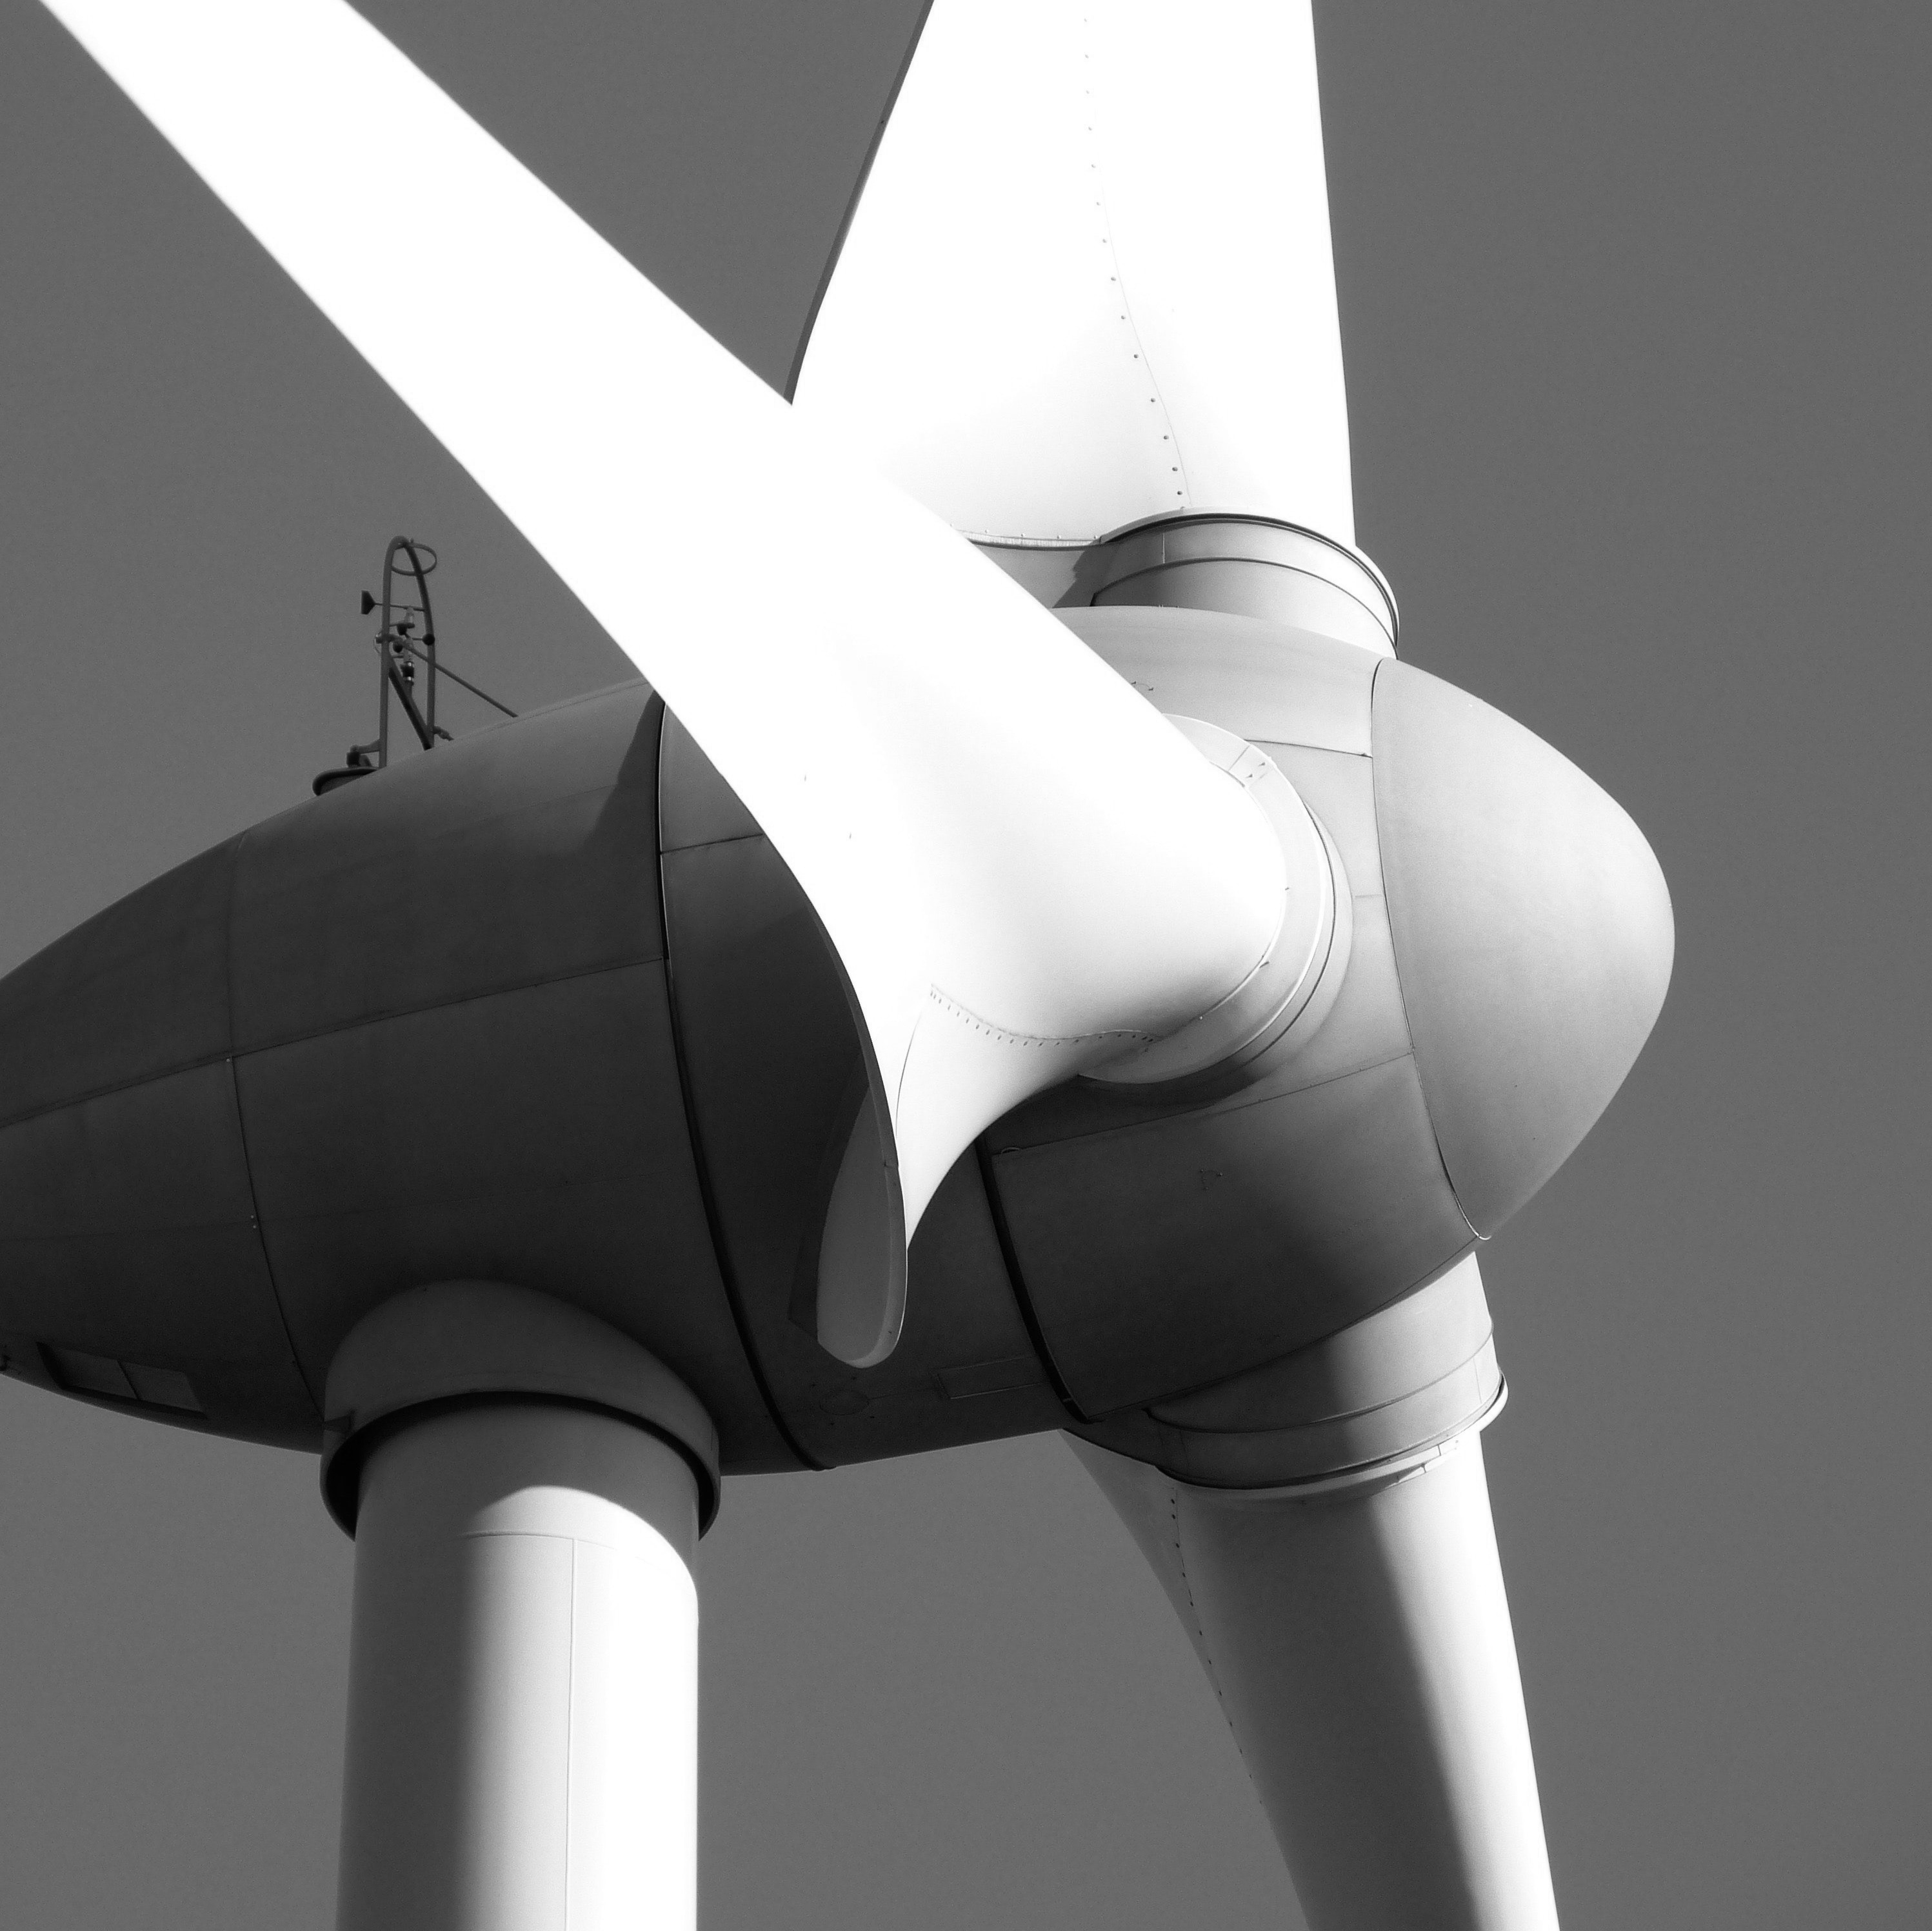
\includegraphics[width=0.4\textwidth]{/home/alameddin/src/tex/phd_thesis/figures/intro/0close-up-propeller-renewable-energy-687692.jpg} \\[0.2cm]
			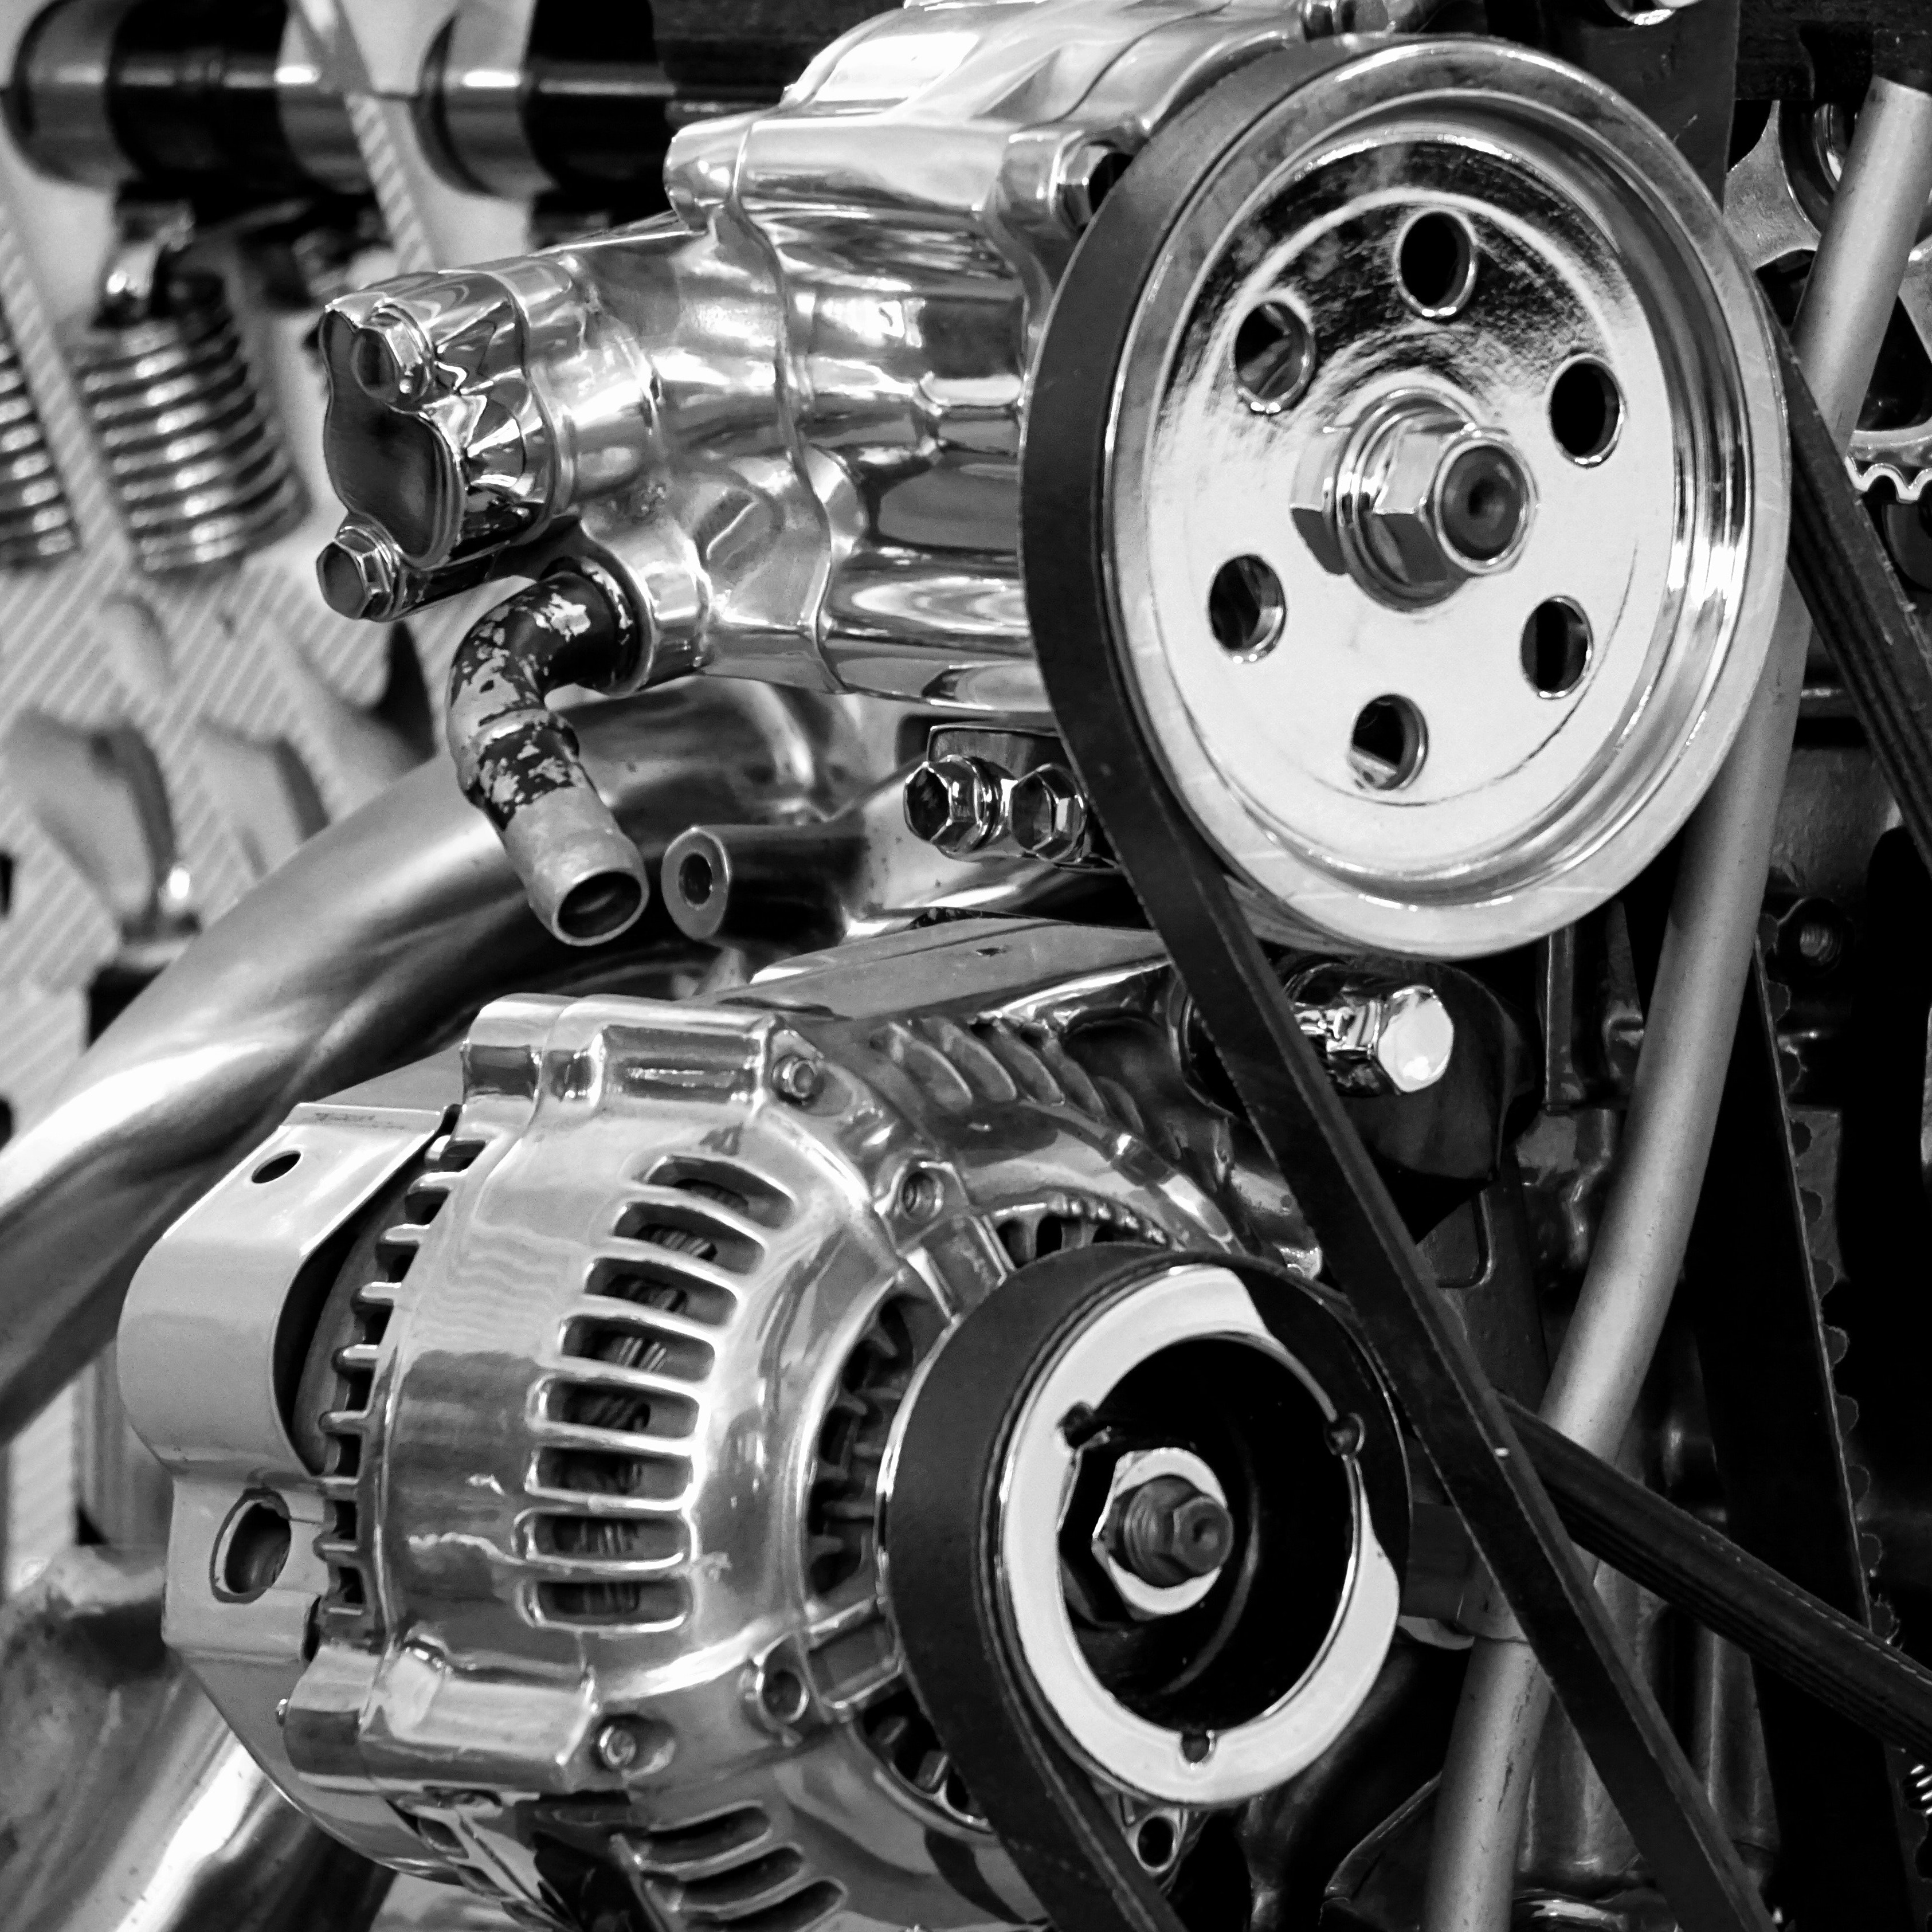
\includegraphics[width=0.4\textwidth]{/home/alameddin/src/tex/phd_thesis/figures/intro/2black-and-white-car-engine-chrome-1905742.jpg} \hspace{0.05cm}			
			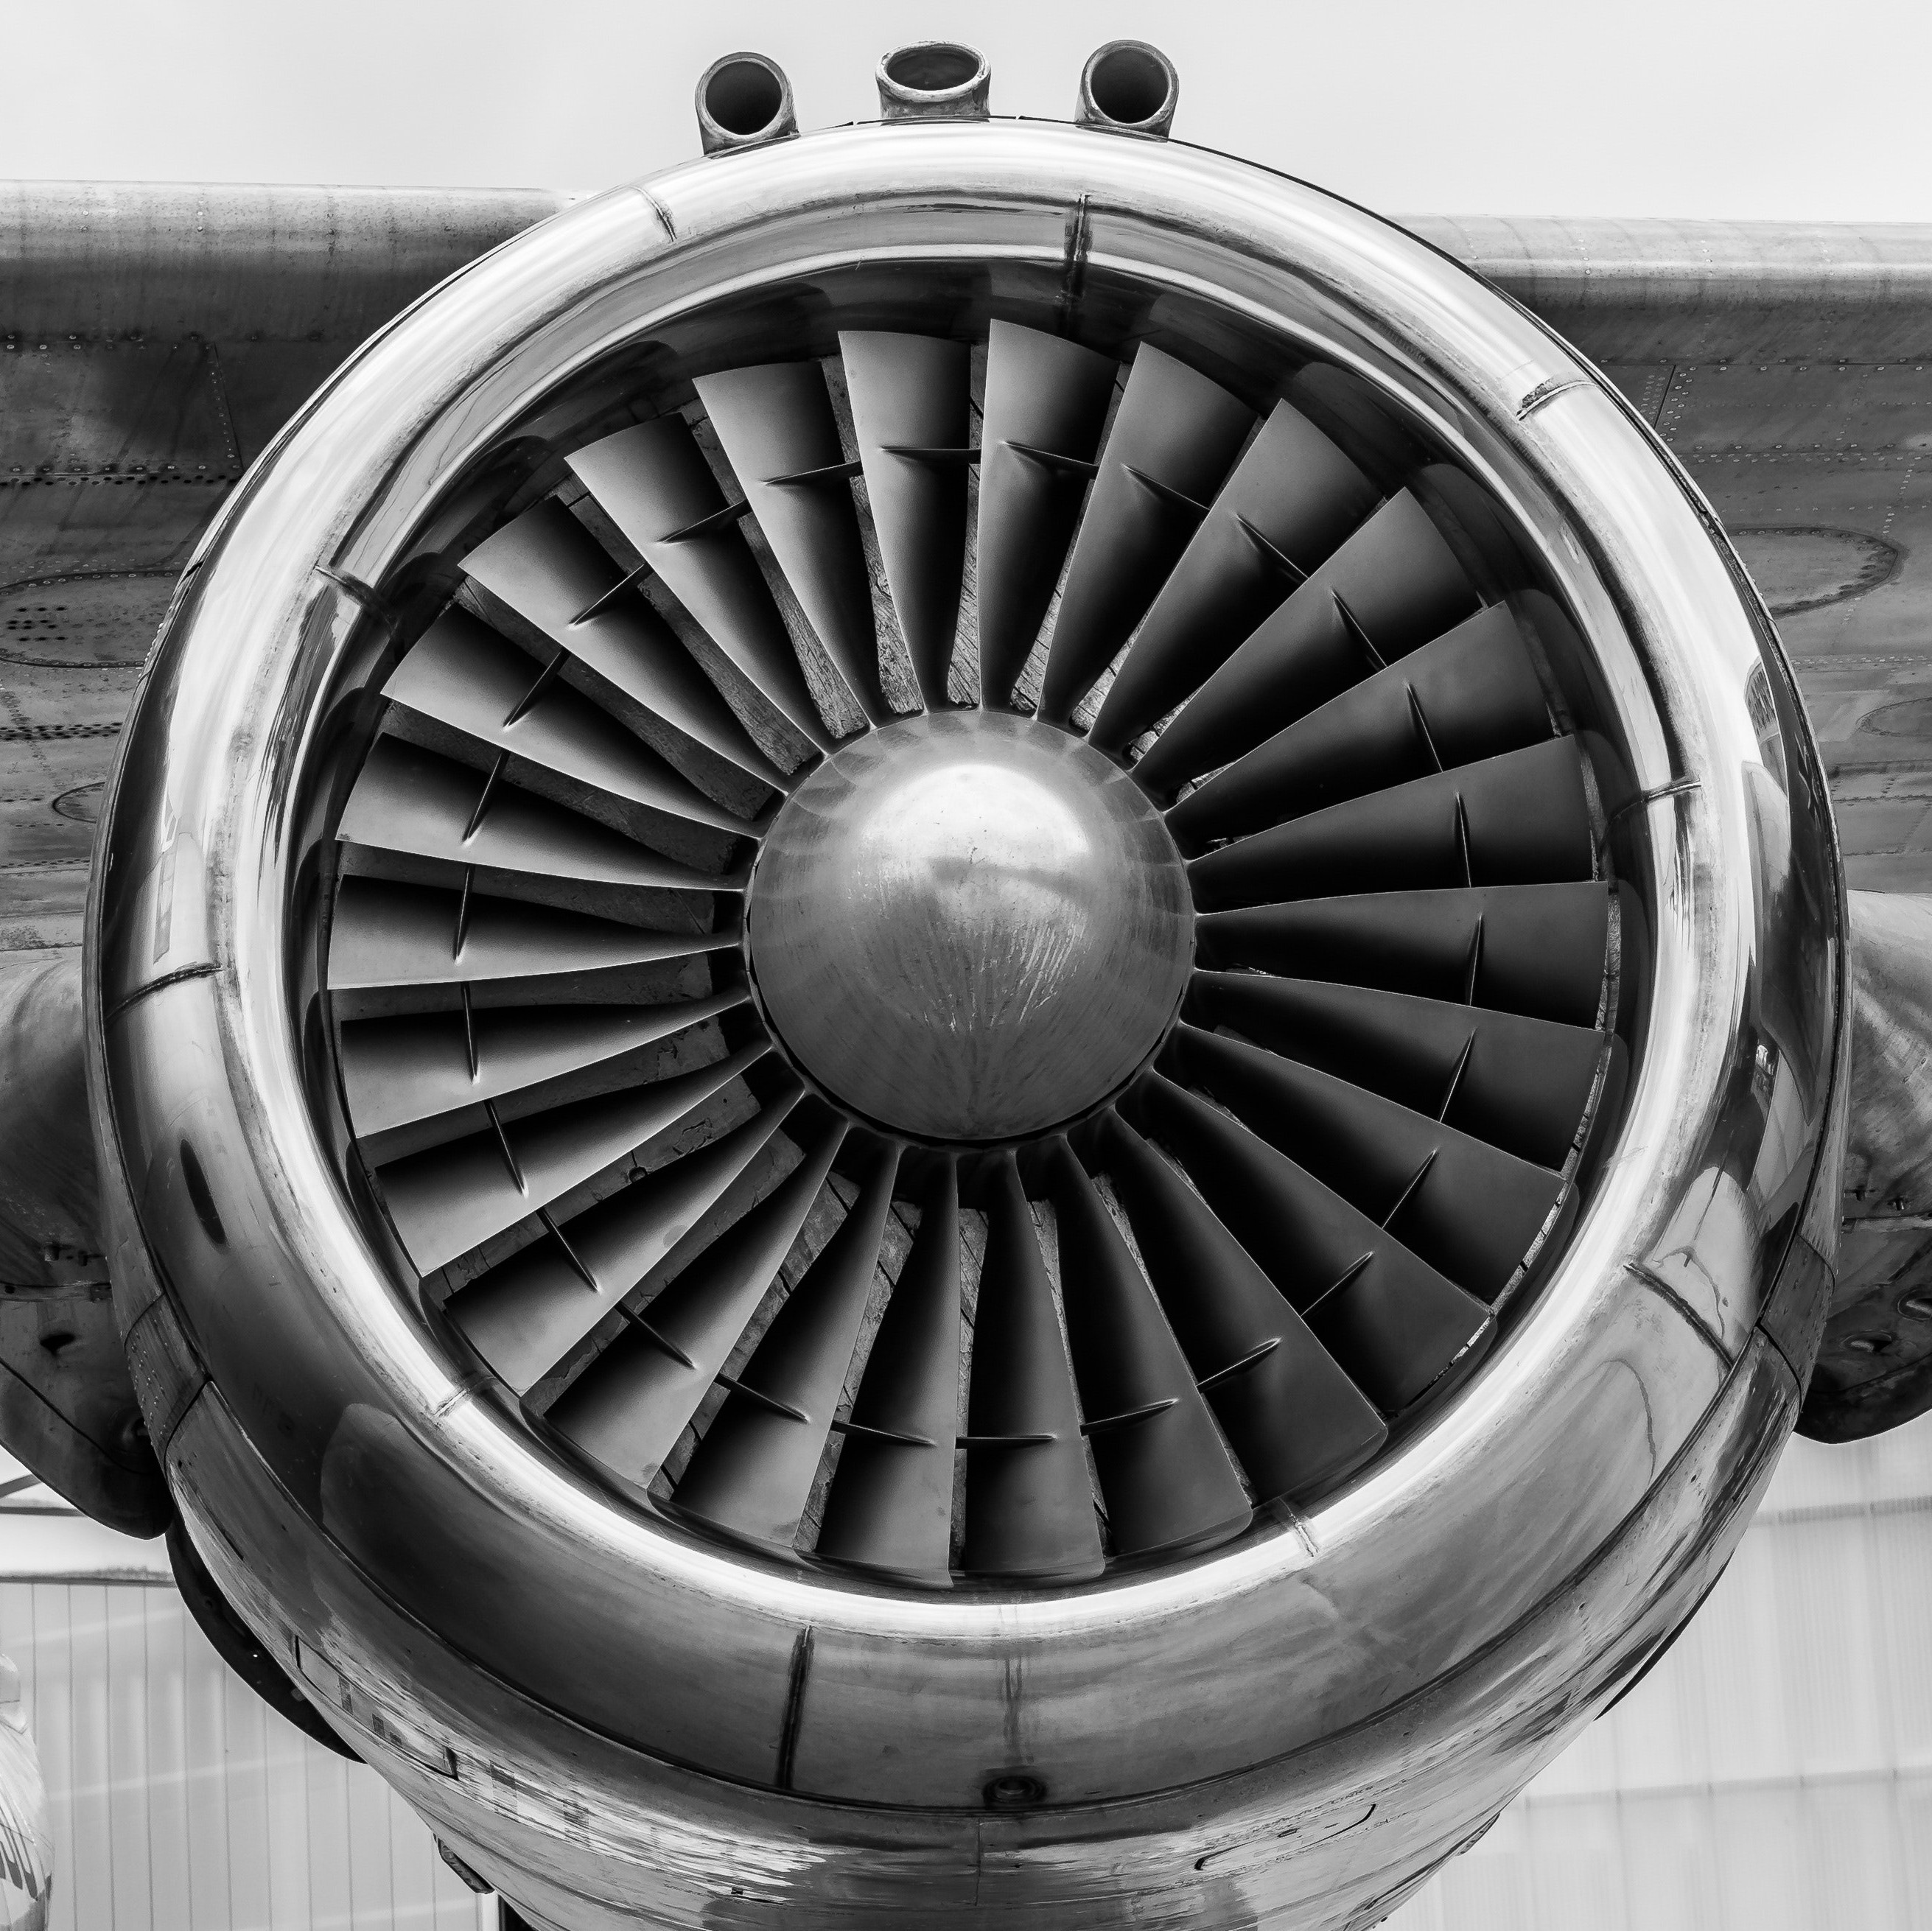
\includegraphics[width=0.4\textwidth]{/home/alameddin/src/tex/phd_thesis/figures/intro/1aeroplane-aircraft-airplane-4594022.jpg}
		\end{itemize}
			
		}{
			\centering
			\uncover<2->{
				\begin{itemize}
					\item Material degradation\\
					{\color{luhBlue} lower load carrying capacity}\\[0.26cm]
					\item Large number of load cycles\\
					{\color{luhBlue} thousands or millions}\\[0.26cm]
					% \item Virtual experiments
					\item Continuum damage model\\
					{\color{luhBlue} $\dot{D} = \d D / \d t$}\\[0.26cm]
%					$\dot{\fq} = \hat{g}{(\phi(\fsigma,\fQ))$
					% \item Macro crack initiation\\[0.5cm]
					\item Computational expense\\ % demand
					{\color{luhBlue} memory and time}
				\end{itemize}
			}
		}
		{\uncover<3->{
			\vspace{0.5cm}
			\begin{block}{ \centering Model order reduction (MOR) techniques}
			\end{block}
		}}
}

\section{Reduced order model for cyclic loading}

\frame[t]{\frametitle{Proper Generalised Decomposition}
	\begin{itemize}
		\item Low-rank approximation\\[-0.7cm]
		\begin{align*}
			\fu(\fx,t) = \sum_{j=1}^{N} {\fv_j}(\fx) \circ \flambda_j(t)
		\end{align*}
		\vfill
		\item Enrichment to ($\mu$) previously generated modes\\[-0.7cm]
		\begin{align*}
			\Delta \fu_{i+1}(\fx,t) = {\fv}_{\color{red}\mu+1}(\fx) \circ \flambda_{\color{red}\mu+1}(t)
		\end{align*}
		\vfill
		\item POD-like update of ($\mu$) previously generated modes\\[-0.7cm]
		\begin{align*}
			\Delta \fu_{i+1}(\fx,t) = \sum_{j=1}^{{\color{red} \mu}} \underbrace{{\fv_j}(\fx)}_{\color{luhBlue} \text{known}} \ \circ \ \Delta \flambda_j(t)
		\end{align*}
	\end{itemize}
}

\section{Challenges and workarounds}

\frame{\frametitle{Semi-incremental extension}
\begin{itemize}
\item The temporal domain is divided into cycles
\item Cycles are simulated consecutively
\vfill
{
	\hspace*{2cm}
		\includegraphics[width=0.5\linewidth]{/home/alameddin/src/tex/phd_thesis/figures/semi_incremental/temporal_scheme_simtech_1.pdf}
}
\item Already generated $\{\lambda_j(t)\}_{j=1}^{\mu}$ are scaled to $\z{t} \in [0,1]$
\item Scaled back to the temporal coordinate of the current cycle
%\item Variable frequencies
\end{itemize}
}

\frame{\frametitle{Semi-incremental extension}
	\begin{itemize}
		\item Continuity of the temporal modes is an issue
		\item Temporal modes are vertically scaled and shifted via \\[-0.8cm]
		\begin{align*}
		&\z{\lambda}_j^{(n+1)}(\z{t}) = m \ \z\lambda_j^{(n)}(\z{t}) + {\color{red} g \ \z{t} + h} \text{\quad with I.C. and B.C.}\\[-0.7cm]
%		& \z{\lambda}_j^{(n+1)}(0) = \z\lambda_j^{(n)}(1) ,
%		\quad
%		\z{\lambda}_j^{(n+1)}(1) = \z{\lambda}_j^{(n+1)}(0).\\[-1cm]
		\end{align*}
		
	\hspace*{2cm}
	\includegraphics[width=0.5\linewidth]{/home/alameddin/src/tex/phd_thesis/figures/semi_incremental/temporal_scheme_simtech_2.pdf}
	\begin{textblock*}{\textwidth}(12mm,0.88\textheight)
	\begin{block}<2>{\centering Variable loading / integration over confined domains \dSmiley}
	\end{block}
	\end{textblock*}
	\end{itemize}
}

\frame{\frametitle{SVD Compression of PGD}
	\begin{itemize}
		\item Large number of modes
		\item Slow temporal update step
		\begin{align*}
		& \mat{\z{A}} \ \T{\z{\mat{\Lambda}}} = \mat{\z{B}}  \\ 
		& \z\mA \in \ffR^{\color{blue} \mu \times \mu} \qquad \mat{\z{B}} \in \ffR^{\color{blue} \mu  \times n_t} \qquad \z{\mat{\Lambda}}=[\Delta\vlambda_{1},\cdots,\Delta\vlambda_{\mu}]
		\end{align*}
		\vfill
		\item Enrichment with a Gram-Schmidt scheme is not optimal
		\item SVD is optimal but expensive to compute
	\end{itemize}
}

\frame[t]{\frametitle{SVD Compression of PGD}
	\begin{itemize}
		\item Given a solution ${\mat{U}} = \mV \ \T{\mat{\Lambda}} \in \ffR^{n\times n_t}$ with\\[-0.9cm]
		\begin{align*}
		\mV=[\vec{v}_1,\cdots,\vec{v}_{\mu}] \in \ffR^{n\times \mu} \qquad \mat{\Lambda}=[\vlambda_1,\cdots,\vlambda_{\mu}] \in \ffR^{n_t \times \mu} 
		\end{align*}
		\vfill
		\item Exploit the outer product format of PGD\\[-0.9cm]
		\begin{align*}
		\mV =  {\color{blue} \mat{Q}_v \ \mat{R}_v }\qquad \mat{\Lambda} = {\color{red} \mat{Q}_\lambda \ \mat{R}_\lambda} 
		\end{align*}
		\vfill
		\item Compute SVD of a small matrix\\[-0.9cm]
		\begin{align*}
		\mat{T} = {\color{blue} \mat{R}_v} \ {\color{red} \T{\mat{R}}_\lambda}\in \ffR^{\mu\times\mu} \qquad \mat{T} \approxeq \hat{\mat{V}} \ \hat{\mat{S}} \ \T{\hat{\mat{\Lambda}}}
		\end{align*}
		\vfill
		\item Solution with a compressed basis\\[-0.9cm]
		\begin{align*}
		{\mat{U}} \approxeq {\color{blue} \mat{Q}_v \ \hat{\mat{V}}} \quad \hat{\mat{S}} \quad {\color{red} \T{\hat{\mat{\Lambda}}} \T{\mat{Q}_\lambda}}
		\end{align*}
\end{itemize}
\begin{textblock*}{\textwidth}(12mm,0.88\textheight)
	\begin{block}<2>{\centering Non-demanding optimal decomposition \dSmiley}
	\end{block}
\end{textblock*}
}

\section{Numerical examples}

\frame{\frametitle{Numerical results}
	\framesubtitle{Viscoplastic viscodamage material}
\begin{itemize}
\item A plate subjected to cyclic loading (Cr-Mo steel at $580^\circ \rm C$)
\begin{figure}
\centering
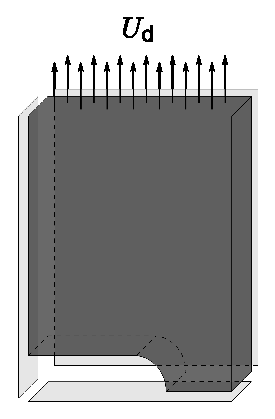
\includegraphics[scale=0.7,clip]{/home/alameddin/src/tex/phd_thesis/figures/3d_plate_1_8.eps}
\end{figure}
\item Plasticity, kinematic and isotropic hardening, damage
\end{itemize}
}

%\begin{minipage}[t]{0.4\textwidth}
%\begin{itemize}
%{\item }
%\vspace{-0.3cm}
%\begin{equation*}
%\begin{split}
%\fsigma & = \ffC \ \fepse \ (1-D) \\
%\fbeta &= C \ \falpha \\
%Y & = \frac{1}{2} \fepse : \ffC \ \fepse
%\end{split}
%\end{equation*}
%\end{itemize}
%\end{minipage}\hfil\begin{minipage}[t]{0.5\textwidth}
%\begin{itemize}
%{\item Evolution equations}
%\vspace{-0.3cm}
%\small
%\begin{equation*}
%\begin{split}
%{\dot{\epst}}^{\rm p} &=  k \ \vol{\Fp}_+^{n} \ \left[\frac{3}{2} \frac{\ftau}{J_{2}(\ftau)} \right] \frac{1}{1-D}\\
%{\dot\alpha} &= k \ \vol{\Fp}_+^{n} \ \left[ \frac{3}{2} \frac{\ftau}{J_{2}(\ftau)} - \frac{a}{C} \fbeta \right] \\
%{\dot{D}} &=  \kd  \vol{\Fd}_+^{\nd}
%\end{split}
%\end{equation*}
%\end{itemize}
%\end{minipage}
%\vspace{0.5cm}

% till here 10 slides

\frame{\frametitle{Model verification}
			\framesubtitle{$ 1884 \cdot 41 \cdot 10 $ DOF}
\vspace{0.6cm} With respect to a modified Newton-Raphson scheme \\[1cm]
\vfill
\twocol{
\centering
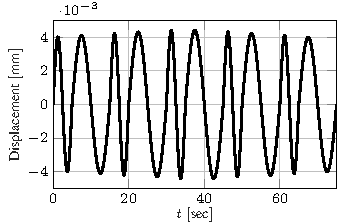
\includegraphics[height=0.55\textheight,width=0.63\textheight]{/home/alameddin/src/tex/phd_thesis/figures/verify/prescribed_displacement.pdf}\\ \hspace{1cm}
{\small Prescribed displacement}
}{
\centering
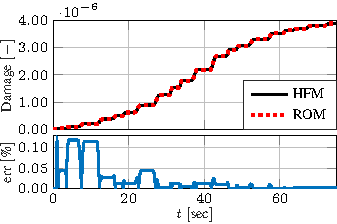
\includegraphics[height=0.55\textheight,width=0.63\textheight]{/home/alameddin/src/tex/phd_thesis/figures/verify/damage_comparison.pdf}\\ \hspace{1cm}
{\small Damage evolution}
}{ }
}
% maximum reaches 12

\frame{\frametitle{Model verification} 
\begin{center}
		$
	\left\lVert {\fe} \right\rVert_{\Omega\times\cI}^2 = \frac{1}{T \ \abs{\Omega}} \intT \intS \fe : \fe \ \d \Omega \d t
	$\\[0.8cm]
\end{center}
	\vfill
	\twocol{
		\centering
		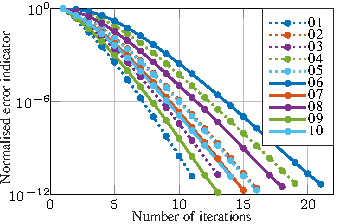
\includegraphics[height=0.52\textheight,width=0.63\textheight]{/home/alameddin/src/tex/phd_thesis/figures/verify/error_indicator.pdf}\\ \hspace{1cm}
{\small 		Error indicator}
	}{
		\centering
		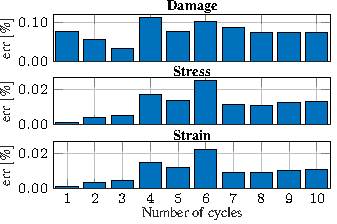
\includegraphics[height=0.54\textheight,width=0.63\textheight]{/home/alameddin/src/tex/phd_thesis/figures/verify/error_space_time.pdf}\\ \hspace{0.6cm}
{\small 		Space-time average relative error}
	}{ }
}

%\frame[c]{\frametitle{Model verification}
%\vspace{0.6cm} Number of modes and iterations\\[1cm]
%	\vfill
%	\twocol{
%		\centering
%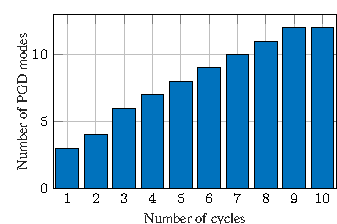
\includegraphics[height=0.53\textheight,width=0.63\textheight]{/home/alameddin/src/tex/phd_thesis/figures/verify/number_of_pgd_modes.pdf}\\ \hspace{1cm}
%{\small 		Number of modes}
%	}{
%		\centering
%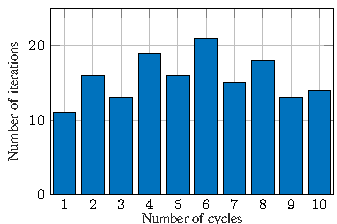
\includegraphics[height=0.53\textheight,width=0.63\textheight]{/home/alameddin/src/tex/phd_thesis/figures/verify/number_of_iterations.pdf}\\ \hspace{1cm}
%{\small 		Number of iterations}
%	}{ }
%}

\frame{\frametitle{Model verification}
\vspace{0.6cm} The first temporal and spatial modes \\[1cm]
	\vfill
	\twocol{
		\centering
		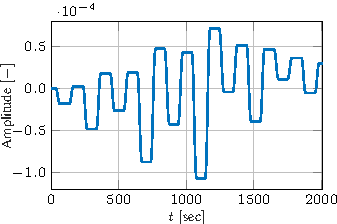
\includegraphics[height=0.54\textheight,width=0.63\textheight]{/home/alameddin/src/tex/phd_thesis/figures/verify/first_temporal_mode.pdf}
	}{
		\centering
		\begin{tikzpicture}[overlay]
		\node (fig1) at (0,2.4)
		{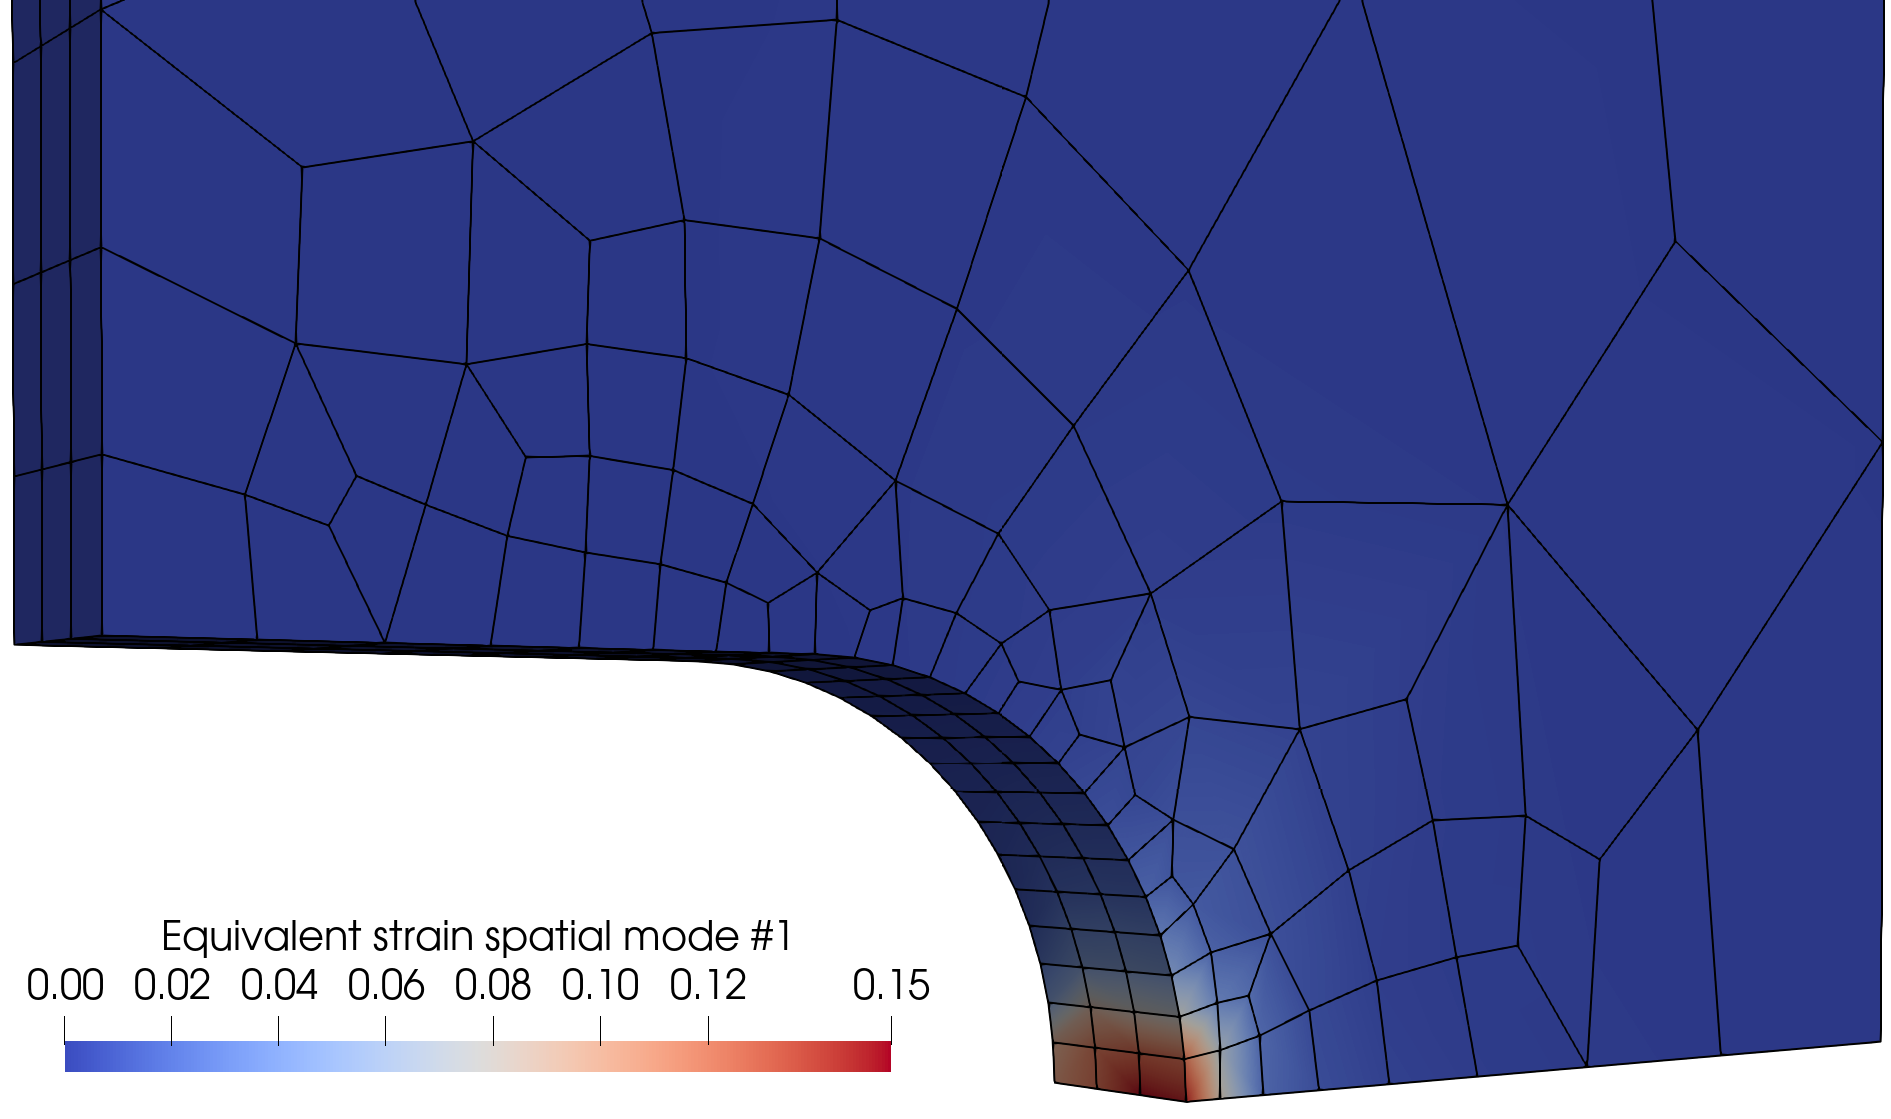
\includegraphics[width=0.8\linewidth,height=0.465\textheight]{/home/alameddin/src/tex/phd_thesis/figures/verify/first_strain_spatial_mode.png}};
		\end{tikzpicture}
	}{ }
	\uncover<2>{\begin{block}{ \centering 12 modes / Speedup factor $\sim 25$ }
	\end{block}}
}

\frame{\frametitle{Variable amplitudes \& frequencies}
	Amplitudes: $[30,90]\cdot10^{-4}\unit{mm}$ \hfill Time periods: $[20,60]\unit{sec}$\\[0.5cm]
	\vfill
	\twocol{
		\centering
		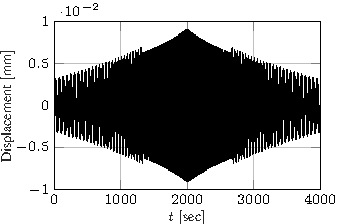
\includegraphics[height=0.5\textheight,width=0.63\textheight]{/home/alameddin/src/tex/phd_thesis/figures/semi_incremental/temporal_scheme_2_1.pdf}\\ \hspace{1cm}
{\small 		Prescribed displacement}
	}{
		\centering
		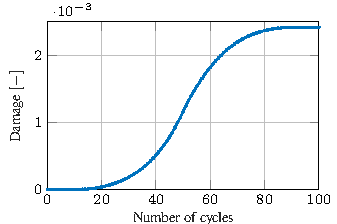
\includegraphics[height=0.5\textheight,width=0.63\textheight]{/home/alameddin/src/tex/phd_thesis/figures/semi_incremental/temporal_scheme_2_2.pdf}\\ \hspace{0.8cm}
{\small 		Damage evolution}
	}{}
}

\frame{\frametitle{Variable amplitudes \& frequencies}
	The growth of the ROB using an SVD scheme\\[0.5cm]
	\vfill
	\twocol{
	\centering
	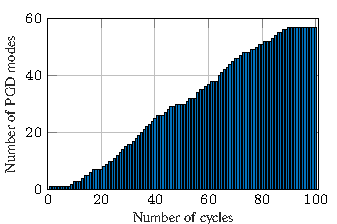
\includegraphics[height=0.5\textheight,width=0.63\textheight]{/home/alameddin/src/tex/phd_thesis/figures/semi_incremental/temporal_scheme_2_5.pdf}\\ \hspace{0.7cm}
{\small 	Gram-Schmidt}
}{
	\centering
	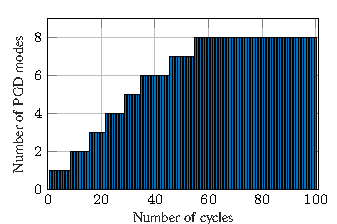
\includegraphics[height=0.5\textheight,width=0.63\textheight]{/home/alameddin/src/tex/phd_thesis/figures/semi_incremental/temporal_scheme_2_4.pdf}\\ \hspace{0.5cm}
{\small 	SVD scheme}
}{}	
}

\frame{\frametitle{Different ortho. schemes} \framesubtitle{$50,547 \cdot 33 \cdot 100$ DOF}
	In case of random loading and fine discretisation\\[0.5cm]
	\vfill
	\twocol{
		\centering
		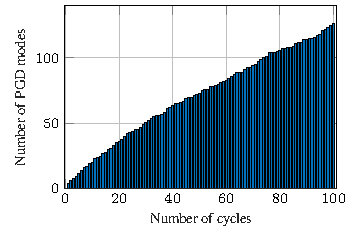
\includegraphics[height=0.5\textheight,width=0.63\textheight]{/home/alameddin/src/tex/phd_thesis/figures/modal_optimisation/mgs_number_of_pgd_modes.pdf}\\ \hspace{0.7cm}
{\small 	Gram-Schmidt}
	}{
		\centering
		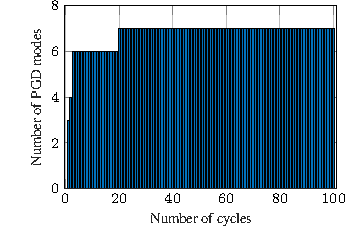
\includegraphics[height=0.5\textheight,width=0.63\textheight]{/home/alameddin/src/tex/phd_thesis/figures/modal_optimisation/excessive_svd_m8_number_of_pgd_modes.pdf}\\ \hspace{0.5cm}
{\small 	SVD scheme}
	}{ }
}

\frame{\frametitle{Different ortho. schemes}
	The required time to update and orthonormalise the modes\\[0.5cm]
	\vfill
	\twocol{
		\centering
		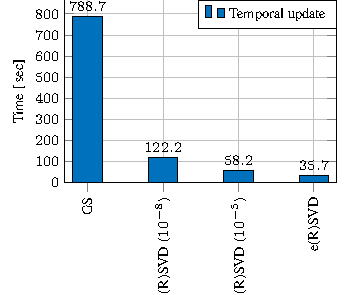
\includegraphics[height=0.5\textheight,width=0.62\textheight]{/home/alameddin/src/tex/phd_thesis/figures/modal_optimisation/temporal_update_timing.pdf}\\
		\hfil Temporal update
	}{
		\centering
		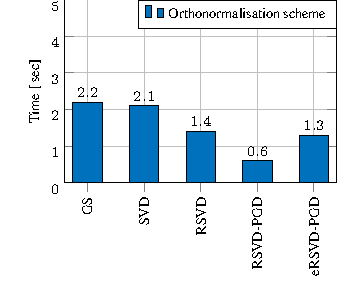
\includegraphics[height=0.5\textheight,width=0.62\textheight]{/home/alameddin/src/tex/phd_thesis/figures/modal_optimisation/orthonormalisation_timing.pdf}\\
		\hfil Orthonormalisation step
	}{ }
}

\frame[t]{\frametitle{Random amplitude loading}
	\framesubtitle{$ 1884 \cdot 41 \cdot 10^4 $ DOF}
	\begin{itemize}
		\item $10^4$ cycles, uniform distribution in $[53,56]\cdot 10^{-2} \unit{mm}$\\[0.5cm]
	\end{itemize}
	\vfill
	\twocol{
		\centering
		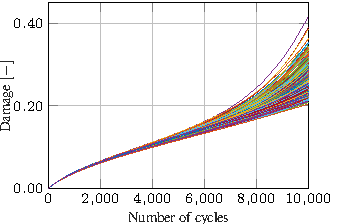
\includegraphics[height=0.51\textheight,width=0.63\textheight]{/home/alameddin/src/tex/phd_thesis/figures/semi_incremental/temporal_scheme_3_1.pdf}\\
		\only<1>{\hspace{0.7cm} \small Different damage realisations}
		\uncover<2->{$\text{Critical damage value } D_{\mathrm{c}}=0.3$\\
		$\ \text{Probability of failure } P_{\mathrm{f}}=5.4\%$}
	}{
		\centering
		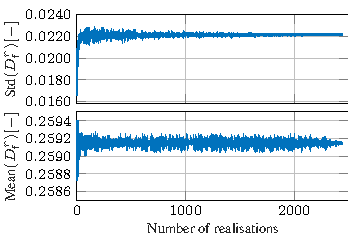
\includegraphics[height=0.5\textheight,width=0.63\textheight]{/home/alameddin/src/tex/phd_thesis/figures/semi_incremental/temporal_scheme_3_2.pdf}\\
		\only<1>{\hspace{0.6cm} \small The mean and STD of $D_f$}		
		\uncover<2->{Requirements:\\ $[15-35]\unit{min}$ and $[1-1.5]\unit{GB}$}
	}{
	\uncover<3>{\begin{block}{ \centering Approx. 10 modes / Time-saving factors $50 \sim 100$}
	\end{block}}
	}
}

\frame{\frametitle{Conclusions}
\vspace{0.5cm}
\begin{itemize}
\item Efficient semi-incremental scheme for damage problems
\item Can handle variable amplitude and frequency loadings
\item Provides a minimal expansion of PGD
\item Most operations are done over decomposed QoI
\item Open-source code: \url{gitlab.com/shadialameddin/romfem}\\[0.3cm]
\end{itemize}
\vfill
\pause
{\begin{block}{ \centering Thank you for your attention}
\end{block}}
}

\end{document}



%TODO Video
%\documentclass[12pt,a4paper]{article}
%\usepackage[utf8]{inputenc}
%\usepackage[T1]{fontenc}
%\usepackage{parskip}
%
%\usepackage{graphicx}
%\usepackage{media9}
%\title{Using media9 to include video and audio files}
%\begin{document}
%	
%	Videos and audios don't play on Overleaf! Download the PDF and open in Acrobat Reader to view. :-)
%	
%	This is an .mp4 file:
%	
%	% using a .mp4; downloaded from https://www.youtube.com/watch?v=-9iXD2-hbJM
%	\includemedia[width=0.6\linewidth,height=0.6\linewidth,activate=pageopen,
%	passcontext,
%	transparent,
%	addresource=penguinschasingbutterfly.mp4,
%	flashvars={source=penguinschasingbutterfly.mp4}
%	]{\includegraphics[width=0.6\linewidth]{penguins}}{VPlayer.swf}
%	
%	This is a YouTube video (needs an Internet connection to view):
%	
%	% using a YouTube video
%	\includemedia[
%	width=0.6\linewidth,height=0.3375\linewidth,
%	activate=pageopen,
%	flashvars={
%		modestbranding=1 % no YT logo in control bar
%		&autohide=1 % controlbar autohide
%		&showinfo=0 % no title and other info before start
%		&rel=0 % no related videos after end
%	}
%	]{\includegraphics[width=0.6\linewidth]{048}}{https://www.youtube.com/v/g8Ejj0T0yG4?rel=0}
%	
%	This is an .mp3 file:
%	%% MP3 downloaded from https://www.sample-videos.com/download-sample-audio.php
%	\includemedia[
%	transparent,
%	passcontext,
%	addresource=SampleAudio.mp3,
%	flashvars={source=SampleAudio.mp3},
%	]{\color{blue}\framebox[0.4\linewidth][c]{Applause}}{APlayer.swf}
%\end{document}